\documentclass[twoside]{book}

% Packages required by doxygen
\usepackage{fixltx2e}
\usepackage{calc}
\usepackage{doxygen}
\usepackage[export]{adjustbox} % also loads graphicx
\usepackage{graphicx}
\usepackage[utf8]{inputenc}
\usepackage{makeidx}
\usepackage{multicol}
\usepackage{multirow}
\PassOptionsToPackage{warn}{textcomp}
\usepackage{textcomp}
\usepackage[nointegrals]{wasysym}
\usepackage[table]{xcolor}

% NLS support packages
\usepackage[ngerman]{babel}

% Font selection
\usepackage[T1]{fontenc}
\usepackage[scaled=.90]{helvet}
\usepackage{courier}
\usepackage{amssymb}
\usepackage{sectsty}
\renewcommand{\familydefault}{\sfdefault}
\allsectionsfont{%
  \fontseries{bc}\selectfont%
  \color{darkgray}%
}
\renewcommand{\DoxyLabelFont}{%
  \fontseries{bc}\selectfont%
  \color{darkgray}%
}
\newcommand{\+}{\discretionary{\mbox{\scriptsize$\hookleftarrow$}}{}{}}

% Page & text layout
\usepackage{geometry}
\geometry{%
  a4paper,%
  top=2.5cm,%
  bottom=2.5cm,%
  left=2.5cm,%
  right=2.5cm%
}
\tolerance=750
\hfuzz=15pt
\hbadness=750
\setlength{\emergencystretch}{15pt}
\setlength{\parindent}{0cm}
\setlength{\parskip}{3ex plus 2ex minus 2ex}
\makeatletter
\renewcommand{\paragraph}{%
  \@startsection{paragraph}{4}{0ex}{-1.0ex}{1.0ex}{%
    \normalfont\normalsize\bfseries\SS@parafont%
  }%
}
\renewcommand{\subparagraph}{%
  \@startsection{subparagraph}{5}{0ex}{-1.0ex}{1.0ex}{%
    \normalfont\normalsize\bfseries\SS@subparafont%
  }%
}
\makeatother

% Headers & footers
\usepackage{fancyhdr}
\pagestyle{fancyplain}
\fancyhead[LE]{\fancyplain{}{\bfseries\thepage}}
\fancyhead[CE]{\fancyplain{}{}}
\fancyhead[RE]{\fancyplain{}{\bfseries\leftmark}}
\fancyhead[LO]{\fancyplain{}{\bfseries\rightmark}}
\fancyhead[CO]{\fancyplain{}{}}
\fancyhead[RO]{\fancyplain{}{\bfseries\thepage}}
\fancyfoot[LE]{\fancyplain{}{}}
\fancyfoot[CE]{\fancyplain{}{}}
\fancyfoot[RE]{\fancyplain{}{\bfseries\scriptsize Erzeugt von Doxygen }}
\fancyfoot[LO]{\fancyplain{}{\bfseries\scriptsize Erzeugt von Doxygen }}
\fancyfoot[CO]{\fancyplain{}{}}
\fancyfoot[RO]{\fancyplain{}{}}
\renewcommand{\footrulewidth}{0.4pt}
\renewcommand{\chaptermark}[1]{%
  \markboth{#1}{}%
}
\renewcommand{\sectionmark}[1]{%
  \markright{\thesection\ #1}%
}

% Indices & bibliography
\usepackage{natbib}
\usepackage[titles]{tocloft}
\setcounter{tocdepth}{3}
\setcounter{secnumdepth}{5}
\makeindex

% Hyperlinks (required, but should be loaded last)
\usepackage{ifpdf}
\ifpdf
  \usepackage[pdftex,pagebackref=true]{hyperref}
\else
  \usepackage[ps2pdf,pagebackref=true]{hyperref}
\fi
\hypersetup{%
  colorlinks=true,%
  linkcolor=blue,%
  citecolor=blue,%
  unicode%
}

% Custom commands
\newcommand{\clearemptydoublepage}{%
  \newpage{\pagestyle{empty}\cleardoublepage}%
}

\usepackage{caption}
\captionsetup{labelsep=space,justification=centering,font={bf},singlelinecheck=off,skip=4pt,position=top}

%===== C O N T E N T S =====

\begin{document}

% Titlepage & ToC
\hypersetup{pageanchor=false,
             bookmarksnumbered=true,
             pdfencoding=unicode
            }
\pagenumbering{alph}
\begin{titlepage}
\vspace*{7cm}
\begin{center}%
{\Large Robot Arm\+\_\+\+Arduino \\[1ex]\large 1.\+0.\+0 }\\
\vspace*{1cm}
{\large Erzeugt von Doxygen 1.8.13}\\
\end{center}
\end{titlepage}
\clearemptydoublepage
\pagenumbering{roman}
\tableofcontents
\clearemptydoublepage
\pagenumbering{arabic}
\hypersetup{pageanchor=true}

%--- Begin generated contents ---
\chapter{Project \+: Robot Arm}
\label{index}\hypertarget{index}{}\hypertarget{index_Intro}{}\section{Intro}\label{index_Intro}

\begin{DoxyItemize}
\item Erklärung \+: Ein Roboterarm der mit W\+L\+A\+N-\/\+Kommunikation gesteuert werden kann, 
\end{DoxyItemize}\hypertarget{index_Program}{}\section{Program}\label{index_Program}

\begin{DoxyItemize}
\item Name des Programms \+: Robot Arm\+\_\+\+Arduino 
\end{DoxyItemize}\hypertarget{index_InOutput}{}\section{In\+Output}\label{index_InOutput}

\begin{DoxyItemize}
\item Input \+: \hyperlink{_arduino__kommentiert_8ino}{Arduino\+\_\+kommentiert.\+ino}
\item Output \+: Ausdrücken die Daten des Files \hyperlink{_arduino__kommentiert_8ino}{Arduino\+\_\+kommentiert.\+ino} 
\end{DoxyItemize}\hypertarget{index_CreateInfo}{}\section{Create\+Info}\label{index_CreateInfo}

\begin{DoxyItemize}
\item Autor \+: Jisoo Choi (3103933), Michael Vogt (4391254), Fany Bowt (4345894)
\begin{DoxyItemize}
\item Datum \+: 23-\/06-\/2017 
\end{DoxyItemize}
\end{DoxyItemize}\hypertarget{index_ModifyInfo}{}\section{Modify\+Info}\label{index_ModifyInfo}

\begin{DoxyItemize}
\item 23-\/06-\/2017\+:
\end{DoxyItemize}
\begin{DoxyEnumerate}
\item die erste Version hochgeladen. 
\end{DoxyEnumerate}
\chapter{Hierarchie-\/\+Verzeichnis}
\section{Class Hierarchy}
This inheritance list is sorted roughly, but not completely, alphabetically\+:\begin{DoxyCompactList}
\item object\begin{DoxyCompactList}
\item \contentsline{section}{F\+I\+N\+A\+L\+\_\+\+G\+U\+I\+\_\+\+W\+L\+A\+N.\+Arduino}{\pageref{class_f_i_n_a_l___g_u_i___w_l_a_n_1_1_arduino}}{}
\item \contentsline{section}{F\+I\+N\+A\+L\+\_\+\+G\+U\+I\+\_\+\+W\+L\+A\+N.\+W\+L\+AN}{\pageref{class_f_i_n_a_l___g_u_i___w_l_a_n_1_1_w_l_a_n}}{}
\end{DoxyCompactList}
\end{DoxyCompactList}

\chapter{Datenstruktur-\/\+Verzeichnis}
\section{Class List}
Here are the classes, structs, unions and interfaces with brief descriptions\+:\begin{DoxyCompactList}
\item\contentsline{section}{\hyperlink{class_f_i_n_a_l___g_u_i___w_l_a_n_1_1_arduino}{F\+I\+N\+A\+L\+\_\+\+G\+U\+I\+\_\+\+W\+L\+A\+N.\+Arduino} }{\pageref{class_f_i_n_a_l___g_u_i___w_l_a_n_1_1_arduino}}{}
\item\contentsline{section}{\hyperlink{class_f_i_n_a_l___g_u_i___w_l_a_n_1_1_w_l_a_n}{F\+I\+N\+A\+L\+\_\+\+G\+U\+I\+\_\+\+W\+L\+A\+N.\+W\+L\+AN} }{\pageref{class_f_i_n_a_l___g_u_i___w_l_a_n_1_1_w_l_a_n}}{}
\end{DoxyCompactList}

\chapter{Datei-\/\+Verzeichnis}
\section{Auflistung der Dateien}
Hier folgt die Aufzählung aller Dateien mit einer Kurzbeschreibung\+:\begin{DoxyCompactList}
\item\contentsline{section}{Arduino\+\_\+kommentiert/\hyperlink{_arduino__kommentiert_8ino}{Arduino\+\_\+kommentiert.\+ino} }{\pageref{_arduino__kommentiert_8ino}}{}
\item\contentsline{section}{Arduino\+\_\+kommentiert/\hyperlink{_dumb_server_8cpp}{Dumb\+Server.\+cpp} }{\pageref{_dumb_server_8cpp}}{}
\item\contentsline{section}{Arduino\+\_\+kommentiert/\hyperlink{_dumb_server_8h}{Dumb\+Server.\+h} }{\pageref{_dumb_server_8h}}{}
\end{DoxyCompactList}

\chapter{Datenstruktur-\/\+Dokumentation}
\hypertarget{class_esp_server}{}\section{Esp\+Server Klassenreferenz}
\label{class_esp_server}\index{Esp\+Server@{Esp\+Server}}


{\ttfamily \#include $<$Dumb\+Server.\+h$>$}



Klassendiagramm für Esp\+Server\+:
% FIG 0


Zusammengehörigkeiten von Esp\+Server\+:
% FIG 1
\subsection*{Öffentliche Methoden}
\begin{DoxyCompactItemize}
\item 
\hyperlink{class_esp_server_afcdc76f5ca68d5049657e5d9d971a1c3}{Esp\+Server} (void)
\item 
void \hyperlink{class_esp_server_a1d032e732d4733905d676ef016fcd43c}{begin} (Stream $\ast$\hyperlink{_arduino__kommentiert_8ino_af690b3a6882292855c4091ede8039998}{esp\+\_\+serial}, const char $\ast$ssid, const char $\ast$pass, uint16\+\_\+t port)
\item 
void \hyperlink{class_esp_server_a55995fd6398892be5768da85dde4f533}{my\+\_\+ip} (char $\ast$buf, size\+\_\+t buflen)
\item 
bool \hyperlink{class_esp_server_a6a25e008ded89de0e4599df7170008fb}{connected} ()
\item 
virtual int \hyperlink{class_esp_server_aad68b4972f6b8426004feeef6e98d02d}{available} ()
\item 
virtual int \hyperlink{class_esp_server_a005a9cd487f4ccb4ccef72197bf263b7}{peek} ()
\item 
virtual int \hyperlink{class_esp_server_ae47512714818b3b9a1d29d2bf1f70fdf}{read} ()
\item 
virtual void \hyperlink{class_esp_server_a05062a3ac7c70a79e991b66789384bf1}{flush} ()
\item 
virtual size\+\_\+t \hyperlink{class_esp_server_a0756c42343195dd1d1aa2f61c9b095bf}{write} (const uint8\+\_\+t $\ast$buffer, size\+\_\+t size)
\item 
size\+\_\+t \hyperlink{class_esp_server_aecc7262ee265fd78affe24f35e49e1bb}{write} (uint8\+\_\+t n)
\item 
size\+\_\+t \hyperlink{class_esp_server_ae3ba71ceb4df9357d8e258efe3e79f4d}{write} (unsigned long n)
\item 
size\+\_\+t \hyperlink{class_esp_server_ac256a11ccc8d32664729a7f5bfc71add}{write} (long n)
\item 
size\+\_\+t \hyperlink{class_esp_server_afde7c57b12659422147d9a5e56b76148}{write} (unsigned int n)
\item 
size\+\_\+t \hyperlink{class_esp_server_a2a49890c886a2b0569b11e02f986f867}{write} (int n)
\end{DoxyCompactItemize}
\subsection*{Private Methoden}
\begin{DoxyCompactItemize}
\item 
void \hyperlink{class_esp_server_a191aa3259094cf1d2c0f22cdfbca9f58}{flush\+\_\+in\+\_\+buff} ()
\item 
void \hyperlink{class_esp_server_aeabfb2610ecfdc26e8ce0e624221067f}{reset} ()
\item 
char \hyperlink{class_esp_server_a3da02efeb5f2cbe3a8a1963e5e7f0a47}{blockread} ()
\item 
void \hyperlink{class_esp_server_a6df2412420218304713dd25715e17198}{connect\+\_\+wifi} (const char $\ast$ssid, const char $\ast$pwd)
\item 
void \hyperlink{class_esp_server_a215752989c25b9819ca06bc8f94845ed}{setup\+\_\+server} (uint16\+\_\+t port)
\item 
void \hyperlink{class_esp_server_a2008f0d315cff00a4bcc1120eeb2dc95}{expect} (char $\ast$msg)
\end{DoxyCompactItemize}
\subsection*{Private Attribute}
\begin{DoxyCompactItemize}
\item 
Stream $\ast$ \hyperlink{class_esp_server_a33166aa92db341d47cdf1776492cca62}{\+\_\+esp\+\_\+serial}
\item 
int \hyperlink{class_esp_server_ab601ba8cdf21497e04e862f22e52c590}{connection\+\_\+id}
\item 
int \hyperlink{class_esp_server_a0cff51089b75a6edf347b86727683e7f}{rem\+\_\+msg\+\_\+len}
\end{DoxyCompactItemize}


\subsection{Ausführliche Beschreibung}


Definiert in Zeile 6 der Datei Dumb\+Server.\+h.



\subsection{Beschreibung der Konstruktoren und Destruktoren}
\mbox{\Hypertarget{class_esp_server_afcdc76f5ca68d5049657e5d9d971a1c3}\label{class_esp_server_afcdc76f5ca68d5049657e5d9d971a1c3}} 
\index{Esp\+Server@{Esp\+Server}!Esp\+Server@{Esp\+Server}}
\index{Esp\+Server@{Esp\+Server}!Esp\+Server@{Esp\+Server}}
\subsubsection{\texorpdfstring{Esp\+Server()}{EspServer()}}
{\footnotesize\ttfamily Esp\+Server\+::\+Esp\+Server (\begin{DoxyParamCaption}\item[{void}]{ }\end{DoxyParamCaption})}



Definiert in Zeile 30 der Datei Dumb\+Server.\+cpp.


\begin{DoxyCode}
31 \{
32   \hyperlink{class_esp_server_a33166aa92db341d47cdf1776492cca62}{\_esp\_serial}= NULL;
33   \hyperlink{class_esp_server_ab601ba8cdf21497e04e862f22e52c590}{connection\_id}= -1;
34   \hyperlink{class_esp_server_a0cff51089b75a6edf347b86727683e7f}{rem\_msg\_len}= 0;
35 \}
\end{DoxyCode}


\subsection{Dokumentation der Elementfunktionen}
\mbox{\Hypertarget{class_esp_server_aad68b4972f6b8426004feeef6e98d02d}\label{class_esp_server_aad68b4972f6b8426004feeef6e98d02d}} 
\index{Esp\+Server@{Esp\+Server}!available@{available}}
\index{available@{available}!Esp\+Server@{Esp\+Server}}
\subsubsection{\texorpdfstring{available()}{available()}}
{\footnotesize\ttfamily int Esp\+Server\+::available (\begin{DoxyParamCaption}{ }\end{DoxyParamCaption})\hspace{0.3cm}{\ttfamily [virtual]}}



Definiert in Zeile 141 der Datei Dumb\+Server.\+cpp.


\begin{DoxyCode}
142 \{
143   \textcolor{keywordtype}{int} ser\_available= \hyperlink{class_esp_server_a33166aa92db341d47cdf1776492cca62}{\_esp\_serial}->available();
144 
145   \textcolor{keywordflow}{if}(\hyperlink{class_esp_server_a0cff51089b75a6edf347b86727683e7f}{rem\_msg\_len}) \{
146     \textcolor{comment}{// There is a message in transit}
147 
148     \textcolor{keywordflow}{return}(min(\hyperlink{class_esp_server_a0cff51089b75a6edf347b86727683e7f}{rem\_msg\_len}, ser\_available));
149   \}
150 
151   \textcolor{keywordflow}{if}(ser\_available) \{
152     \textcolor{keywordtype}{char} bte= \hyperlink{class_esp_server_a33166aa92db341d47cdf1776492cca62}{\_esp\_serial}->peek();
153 
154     \textcolor{comment}{/* CONNECT/DISCONNECT messages}
155 \textcolor{comment}{     * start with a number */}
156     \textcolor{keywordflow}{if}(bte >= \textcolor{charliteral}{'0'} && bte <= \textcolor{charliteral}{'9'}) \{
157       \textcolor{comment}{/* Read the connection ID and skip}
158 \textcolor{comment}{       * to the first part of the command */}
159       \textcolor{keywordtype}{int} \textcolor{keywordtype}{id}= \hyperlink{class_esp_server_a33166aa92db341d47cdf1776492cca62}{\_esp\_serial}->parseInt();
160 
161       \hyperlink{class_esp_server_a2008f0d315cff00a4bcc1120eeb2dc95}{expect}((\textcolor{keywordtype}{char} *)\textcolor{stringliteral}{",C"});
162 
163       \textcolor{comment}{/* Read the character that lets us determine}
164 \textcolor{comment}{       * if a connection was opened or closed */}
165       \textcolor{keywordtype}{char} cmd= \hyperlink{class_esp_server_a3da02efeb5f2cbe3a8a1963e5e7f0a47}{blockread}();
166 
167       \textcolor{keywordflow}{if}(cmd == \textcolor{charliteral}{'O'}) \{
168         \textcolor{comment}{// Command is ?,CONNECT}
169 
170         \textcolor{keywordflow}{if}(\hyperlink{class_esp_server_ab601ba8cdf21497e04e862f22e52c590}{connection\_id} >= 0) \{
171           \textcolor{comment}{/* Only allow one open connection,}
172 \textcolor{comment}{           * close the new one */}
173 
174           \hyperlink{class_esp_server_a33166aa92db341d47cdf1776492cca62}{\_esp\_serial}->print(\textcolor{stringliteral}{"AT+CIPCLOSE="});
175           \hyperlink{class_esp_server_a33166aa92db341d47cdf1776492cca62}{\_esp\_serial}->println(\textcolor{keywordtype}{id});
176         \}
177         \textcolor{keywordflow}{else} \{
178           \hyperlink{class_esp_server_ab601ba8cdf21497e04e862f22e52c590}{connection\_id}= id;
179         \}
180       \}
181 
182       \textcolor{keywordflow}{if}(cmd == \textcolor{charliteral}{'L'}) \{
183         \textcolor{comment}{// Command is ?,CLOSED}
184 
185         \textcolor{keywordflow}{if}(\textcolor{keywordtype}{id} == \hyperlink{class_esp_server_ab601ba8cdf21497e04e862f22e52c590}{connection\_id}) \{
186           \hyperlink{class_esp_server_ab601ba8cdf21497e04e862f22e52c590}{connection\_id}= -1;
187         \}
188       \}
189 
190       \hyperlink{class_esp_server_a2008f0d315cff00a4bcc1120eeb2dc95}{expect}((\textcolor{keywordtype}{char} *)\textcolor{stringliteral}{"\(\backslash\)r\(\backslash\)n"});
191     \}
192     \textcolor{keywordflow}{else} \textcolor{keywordflow}{if}(bte == \textcolor{charliteral}{'+'}) \{
193       \textcolor{keywordtype}{char} cmd[5]= \{0\};
194       \hyperlink{class_esp_server_a33166aa92db341d47cdf1776492cca62}{\_esp\_serial}->readBytes(cmd, 4);
195 
196       \textcolor{keywordtype}{int} \textcolor{keywordtype}{id}= \hyperlink{class_esp_server_a33166aa92db341d47cdf1776492cca62}{\_esp\_serial}->parseInt();
197       \textcolor{keywordtype}{int} len= \hyperlink{class_esp_server_a33166aa92db341d47cdf1776492cca62}{\_esp\_serial}->parseInt();
198 
199       \hyperlink{class_esp_server_a2008f0d315cff00a4bcc1120eeb2dc95}{expect}((\textcolor{keywordtype}{char} *)\textcolor{stringliteral}{":"});
200 
201       \textcolor{keywordflow}{if}(\textcolor{keywordtype}{id} == \hyperlink{class_esp_server_ab601ba8cdf21497e04e862f22e52c590}{connection\_id}) \{
202         \hyperlink{class_esp_server_a0cff51089b75a6edf347b86727683e7f}{rem\_msg\_len}= len;
203       \}
204     \}
205     \textcolor{keywordflow}{else} \{
206       \hyperlink{class_esp_server_a33166aa92db341d47cdf1776492cca62}{\_esp\_serial}->read();
207     \}
208   \}
209 
210 
211   \textcolor{keywordflow}{return}(0);
212 \}
\end{DoxyCode}
Hier ist ein Graph, der zeigt, was diese Funktion aufruft\+:
% FIG 2
Hier ist ein Graph der zeigt, wo diese Funktion aufgerufen wird\+:
% FIG 3
\mbox{\Hypertarget{class_esp_server_a1d032e732d4733905d676ef016fcd43c}\label{class_esp_server_a1d032e732d4733905d676ef016fcd43c}} 
\index{Esp\+Server@{Esp\+Server}!begin@{begin}}
\index{begin@{begin}!Esp\+Server@{Esp\+Server}}
\subsubsection{\texorpdfstring{begin()}{begin()}}
{\footnotesize\ttfamily void Esp\+Server\+::begin (\begin{DoxyParamCaption}\item[{Stream $\ast$}]{esp\+\_\+serial,  }\item[{const char $\ast$}]{ssid,  }\item[{const char $\ast$}]{pass,  }\item[{uint16\+\_\+t}]{port }\end{DoxyParamCaption})}



Definiert in Zeile 37 der Datei Dumb\+Server.\+cpp.


\begin{DoxyCode}
38 \{
39   \hyperlink{class_esp_server_a33166aa92db341d47cdf1776492cca62}{\_esp\_serial}= \hyperlink{_arduino__kommentiert_8ino_af690b3a6882292855c4091ede8039998}{esp\_serial};
40   \hyperlink{class_esp_server_a33166aa92db341d47cdf1776492cca62}{\_esp\_serial}->setTimeout(60000);
41 
42   \hyperlink{class_esp_server_aeabfb2610ecfdc26e8ce0e624221067f}{reset}();
43   \hyperlink{class_esp_server_a6df2412420218304713dd25715e17198}{connect\_wifi}(ssid, pass);
44   \hyperlink{class_esp_server_a215752989c25b9819ca06bc8f94845ed}{setup\_server}(port);
45 \}
\end{DoxyCode}
Hier ist ein Graph, der zeigt, was diese Funktion aufruft\+:
% FIG 4
Hier ist ein Graph der zeigt, wo diese Funktion aufgerufen wird\+:
% FIG 5
\mbox{\Hypertarget{class_esp_server_a3da02efeb5f2cbe3a8a1963e5e7f0a47}\label{class_esp_server_a3da02efeb5f2cbe3a8a1963e5e7f0a47}} 
\index{Esp\+Server@{Esp\+Server}!blockread@{blockread}}
\index{blockread@{blockread}!Esp\+Server@{Esp\+Server}}
\subsubsection{\texorpdfstring{blockread()}{blockread()}}
{\footnotesize\ttfamily char Esp\+Server\+::blockread (\begin{DoxyParamCaption}{ }\end{DoxyParamCaption})\hspace{0.3cm}{\ttfamily [private]}}



Definiert in Zeile 54 der Datei Dumb\+Server.\+cpp.


\begin{DoxyCode}
55 \{
56   \textcolor{keywordflow}{while}(!\hyperlink{class_esp_server_a33166aa92db341d47cdf1776492cca62}{\_esp\_serial}->available());
57 
58   \textcolor{keywordflow}{return}(\hyperlink{class_esp_server_a33166aa92db341d47cdf1776492cca62}{\_esp\_serial}->read());
59 \}
\end{DoxyCode}
Hier ist ein Graph der zeigt, wo diese Funktion aufgerufen wird\+:
% FIG 6
\mbox{\Hypertarget{class_esp_server_a6df2412420218304713dd25715e17198}\label{class_esp_server_a6df2412420218304713dd25715e17198}} 
\index{Esp\+Server@{Esp\+Server}!connect\+\_\+wifi@{connect\+\_\+wifi}}
\index{connect\+\_\+wifi@{connect\+\_\+wifi}!Esp\+Server@{Esp\+Server}}
\subsubsection{\texorpdfstring{connect\+\_\+wifi()}{connect\_wifi()}}
{\footnotesize\ttfamily void Esp\+Server\+::connect\+\_\+wifi (\begin{DoxyParamCaption}\item[{const char $\ast$}]{ssid,  }\item[{const char $\ast$}]{pwd }\end{DoxyParamCaption})\hspace{0.3cm}{\ttfamily [private]}}



Definiert in Zeile 87 der Datei Dumb\+Server.\+cpp.


\begin{DoxyCode}
88 \{
89   \textcolor{comment}{// Set station mode}
90   \hyperlink{class_esp_server_a33166aa92db341d47cdf1776492cca62}{\_esp\_serial}->println(\textcolor{stringliteral}{"AT+CWMODE\_CUR=1"});
91   \hyperlink{class_esp_server_a2008f0d315cff00a4bcc1120eeb2dc95}{expect}(\hyperlink{_dumb_server_8cpp_a62497fcb12b1cedd5fdfbc0755508d87}{ESP\_SUCESS\_OK});
92 
93   \textcolor{comment}{// Connect to AP}
94   \hyperlink{class_esp_server_a33166aa92db341d47cdf1776492cca62}{\_esp\_serial}->print(\textcolor{stringliteral}{"AT+CWJAP\_CUR=\(\backslash\)""});
95   \hyperlink{class_esp_server_a33166aa92db341d47cdf1776492cca62}{\_esp\_serial}->print(ssid);
96   \hyperlink{class_esp_server_a33166aa92db341d47cdf1776492cca62}{\_esp\_serial}->print(\textcolor{stringliteral}{"\(\backslash\)",\(\backslash\)""});
97   \hyperlink{class_esp_server_a33166aa92db341d47cdf1776492cca62}{\_esp\_serial}->print(pwd);
98   \hyperlink{class_esp_server_a33166aa92db341d47cdf1776492cca62}{\_esp\_serial}->println(\textcolor{stringliteral}{"\(\backslash\)""});
99   \hyperlink{class_esp_server_a2008f0d315cff00a4bcc1120eeb2dc95}{expect}(\hyperlink{_dumb_server_8cpp_a62497fcb12b1cedd5fdfbc0755508d87}{ESP\_SUCESS\_OK});
100 
101   \textcolor{comment}{// Get an IP using DHCP}
102   \hyperlink{class_esp_server_a33166aa92db341d47cdf1776492cca62}{\_esp\_serial}->println(\textcolor{stringliteral}{"AT+CIFSR"});
103   \hyperlink{class_esp_server_a2008f0d315cff00a4bcc1120eeb2dc95}{expect}(\hyperlink{_dumb_server_8cpp_a62497fcb12b1cedd5fdfbc0755508d87}{ESP\_SUCESS\_OK});
104 \}
\end{DoxyCode}
Hier ist ein Graph, der zeigt, was diese Funktion aufruft\+:
% FIG 7
Hier ist ein Graph der zeigt, wo diese Funktion aufgerufen wird\+:
% FIG 8
\mbox{\Hypertarget{class_esp_server_a6a25e008ded89de0e4599df7170008fb}\label{class_esp_server_a6a25e008ded89de0e4599df7170008fb}} 
\index{Esp\+Server@{Esp\+Server}!connected@{connected}}
\index{connected@{connected}!Esp\+Server@{Esp\+Server}}
\subsubsection{\texorpdfstring{connected()}{connected()}}
{\footnotesize\ttfamily bool Esp\+Server\+::connected (\begin{DoxyParamCaption}{ }\end{DoxyParamCaption})}



Definiert in Zeile 130 der Datei Dumb\+Server.\+cpp.


\begin{DoxyCode}
131 \{
132   \textcolor{comment}{/* available() will, as a side-effect check if}
133 \textcolor{comment}{   * the connection status changed */}
134   \hyperlink{class_esp_server_aad68b4972f6b8426004feeef6e98d02d}{available}();
135 
136   \textcolor{comment}{/* Return true if there is currently a}
137 \textcolor{comment}{   * client connected */}
138   \textcolor{keywordflow}{return}(\hyperlink{class_esp_server_ab601ba8cdf21497e04e862f22e52c590}{connection\_id} >= 0);
139 \}
\end{DoxyCode}
Hier ist ein Graph, der zeigt, was diese Funktion aufruft\+:
% FIG 9
Hier ist ein Graph der zeigt, wo diese Funktion aufgerufen wird\+:
% FIG 10
\mbox{\Hypertarget{class_esp_server_a2008f0d315cff00a4bcc1120eeb2dc95}\label{class_esp_server_a2008f0d315cff00a4bcc1120eeb2dc95}} 
\index{Esp\+Server@{Esp\+Server}!expect@{expect}}
\index{expect@{expect}!Esp\+Server@{Esp\+Server}}
\subsubsection{\texorpdfstring{expect()}{expect()}}
{\footnotesize\ttfamily void Esp\+Server\+::expect (\begin{DoxyParamCaption}\item[{char $\ast$}]{msg }\end{DoxyParamCaption})\hspace{0.3cm}{\ttfamily [private]}}



Definiert in Zeile 61 der Datei Dumb\+Server.\+cpp.


\begin{DoxyCode}
62 \{
63   \textcolor{keywordtype}{char} *exp= msg;
64 
65   \textcolor{keywordflow}{while}(*exp) \{
66     \textcolor{keywordflow}{if} (\hyperlink{class_esp_server_a3da02efeb5f2cbe3a8a1963e5e7f0a47}{blockread}() != *exp) \{
67       exp= msg;
68     \}
69     \textcolor{keywordflow}{else} \{
70       exp++;
71     \}
72   \}
73 \}
\end{DoxyCode}
Hier ist ein Graph, der zeigt, was diese Funktion aufruft\+:
% FIG 11
Hier ist ein Graph der zeigt, wo diese Funktion aufgerufen wird\+:
% FIG 12
\mbox{\Hypertarget{class_esp_server_a05062a3ac7c70a79e991b66789384bf1}\label{class_esp_server_a05062a3ac7c70a79e991b66789384bf1}} 
\index{Esp\+Server@{Esp\+Server}!flush@{flush}}
\index{flush@{flush}!Esp\+Server@{Esp\+Server}}
\subsubsection{\texorpdfstring{flush()}{flush()}}
{\footnotesize\ttfamily void Esp\+Server\+::flush (\begin{DoxyParamCaption}{ }\end{DoxyParamCaption})\hspace{0.3cm}{\ttfamily [virtual]}}



Definiert in Zeile 236 der Datei Dumb\+Server.\+cpp.


\begin{DoxyCode}
237 \{
238   \hyperlink{class_esp_server_a33166aa92db341d47cdf1776492cca62}{\_esp\_serial}->flush();
239 \}
\end{DoxyCode}
\mbox{\Hypertarget{class_esp_server_a191aa3259094cf1d2c0f22cdfbca9f58}\label{class_esp_server_a191aa3259094cf1d2c0f22cdfbca9f58}} 
\index{Esp\+Server@{Esp\+Server}!flush\+\_\+in\+\_\+buff@{flush\+\_\+in\+\_\+buff}}
\index{flush\+\_\+in\+\_\+buff@{flush\+\_\+in\+\_\+buff}!Esp\+Server@{Esp\+Server}}
\subsubsection{\texorpdfstring{flush\+\_\+in\+\_\+buff()}{flush\_in\_buff()}}
{\footnotesize\ttfamily void Esp\+Server\+::flush\+\_\+in\+\_\+buff (\begin{DoxyParamCaption}{ }\end{DoxyParamCaption})\hspace{0.3cm}{\ttfamily [private]}}



Definiert in Zeile 47 der Datei Dumb\+Server.\+cpp.


\begin{DoxyCode}
48 \{
49   \textcolor{keywordflow}{while}(\hyperlink{class_esp_server_a33166aa92db341d47cdf1776492cca62}{\_esp\_serial}->available()) \{
50     \hyperlink{class_esp_server_a33166aa92db341d47cdf1776492cca62}{\_esp\_serial}->read();
51   \}
52 \}
\end{DoxyCode}
Hier ist ein Graph der zeigt, wo diese Funktion aufgerufen wird\+:
% FIG 13
\mbox{\Hypertarget{class_esp_server_a55995fd6398892be5768da85dde4f533}\label{class_esp_server_a55995fd6398892be5768da85dde4f533}} 
\index{Esp\+Server@{Esp\+Server}!my\+\_\+ip@{my\+\_\+ip}}
\index{my\+\_\+ip@{my\+\_\+ip}!Esp\+Server@{Esp\+Server}}
\subsubsection{\texorpdfstring{my\+\_\+ip()}{my\_ip()}}
{\footnotesize\ttfamily void Esp\+Server\+::my\+\_\+ip (\begin{DoxyParamCaption}\item[{char $\ast$}]{buf,  }\item[{size\+\_\+t}]{buflen }\end{DoxyParamCaption})}



Definiert in Zeile 119 der Datei Dumb\+Server.\+cpp.


\begin{DoxyCode}
120 \{
121   \hyperlink{class_esp_server_a33166aa92db341d47cdf1776492cca62}{\_esp\_serial}->println(\textcolor{stringliteral}{"AT+CIPSTA\_CUR?"});
122   \hyperlink{class_esp_server_a2008f0d315cff00a4bcc1120eeb2dc95}{expect}(\hyperlink{_dumb_server_8cpp_a4a3c8fcc7b628944ea321ad928a00bd9}{ESP\_SUCESS\_IPQ});
123 
124   memset(buf, 0, buflen);
125   \hyperlink{class_esp_server_a33166aa92db341d47cdf1776492cca62}{\_esp\_serial}->readBytesUntil(\textcolor{charliteral}{'"'}, buf, buflen - 1);
126 
127   \hyperlink{class_esp_server_a2008f0d315cff00a4bcc1120eeb2dc95}{expect}(\hyperlink{_dumb_server_8cpp_a62497fcb12b1cedd5fdfbc0755508d87}{ESP\_SUCESS\_OK});
128 \}
\end{DoxyCode}
Hier ist ein Graph, der zeigt, was diese Funktion aufruft\+:
% FIG 14
Hier ist ein Graph der zeigt, wo diese Funktion aufgerufen wird\+:
% FIG 15
\mbox{\Hypertarget{class_esp_server_a005a9cd487f4ccb4ccef72197bf263b7}\label{class_esp_server_a005a9cd487f4ccb4ccef72197bf263b7}} 
\index{Esp\+Server@{Esp\+Server}!peek@{peek}}
\index{peek@{peek}!Esp\+Server@{Esp\+Server}}
\subsubsection{\texorpdfstring{peek()}{peek()}}
{\footnotesize\ttfamily int Esp\+Server\+::peek (\begin{DoxyParamCaption}{ }\end{DoxyParamCaption})\hspace{0.3cm}{\ttfamily [virtual]}}



Definiert in Zeile 214 der Datei Dumb\+Server.\+cpp.


\begin{DoxyCode}
215 \{
216   \textcolor{keywordflow}{if}(\hyperlink{class_esp_server_aad68b4972f6b8426004feeef6e98d02d}{available}()) \{
217     \textcolor{keywordflow}{return}(\hyperlink{class_esp_server_a33166aa92db341d47cdf1776492cca62}{\_esp\_serial}->peek());
218   \}
219   \textcolor{keywordflow}{else} \{
220     \textcolor{keywordflow}{return}(-1);
221   \}
222 \}
\end{DoxyCode}
Hier ist ein Graph, der zeigt, was diese Funktion aufruft\+:
% FIG 16
\mbox{\Hypertarget{class_esp_server_ae47512714818b3b9a1d29d2bf1f70fdf}\label{class_esp_server_ae47512714818b3b9a1d29d2bf1f70fdf}} 
\index{Esp\+Server@{Esp\+Server}!read@{read}}
\index{read@{read}!Esp\+Server@{Esp\+Server}}
\subsubsection{\texorpdfstring{read()}{read()}}
{\footnotesize\ttfamily int Esp\+Server\+::read (\begin{DoxyParamCaption}{ }\end{DoxyParamCaption})\hspace{0.3cm}{\ttfamily [virtual]}}



Definiert in Zeile 224 der Datei Dumb\+Server.\+cpp.


\begin{DoxyCode}
225 \{
226   \textcolor{keywordflow}{if}(\hyperlink{class_esp_server_aad68b4972f6b8426004feeef6e98d02d}{available}()) \{
227     \hyperlink{class_esp_server_a0cff51089b75a6edf347b86727683e7f}{rem\_msg\_len} -= 1;
228 
229     \textcolor{keywordflow}{return}(\hyperlink{class_esp_server_a33166aa92db341d47cdf1776492cca62}{\_esp\_serial}->read());
230   \}
231   \textcolor{keywordflow}{else} \{
232     \textcolor{keywordflow}{return}(-1);
233   \}
234 \}
\end{DoxyCode}
Hier ist ein Graph, der zeigt, was diese Funktion aufruft\+:
% FIG 17
\mbox{\Hypertarget{class_esp_server_aeabfb2610ecfdc26e8ce0e624221067f}\label{class_esp_server_aeabfb2610ecfdc26e8ce0e624221067f}} 
\index{Esp\+Server@{Esp\+Server}!reset@{reset}}
\index{reset@{reset}!Esp\+Server@{Esp\+Server}}
\subsubsection{\texorpdfstring{reset()}{reset()}}
{\footnotesize\ttfamily void Esp\+Server\+::reset (\begin{DoxyParamCaption}{ }\end{DoxyParamCaption})\hspace{0.3cm}{\ttfamily [private]}}



Definiert in Zeile 75 der Datei Dumb\+Server.\+cpp.


\begin{DoxyCode}
76 \{
77   \hyperlink{class_esp_server_a33166aa92db341d47cdf1776492cca62}{\_esp\_serial}->println(\textcolor{stringliteral}{"AT+RST"});
78   \hyperlink{class_esp_server_a2008f0d315cff00a4bcc1120eeb2dc95}{expect}(\hyperlink{_dumb_server_8cpp_af9850325c242ec48a5d70923c6147de5}{ESP\_SUCESS\_READY});
79 
80   \hyperlink{class_esp_server_a191aa3259094cf1d2c0f22cdfbca9f58}{flush\_in\_buff}();
81 
82   \textcolor{comment}{// Disable command echo}
83   \hyperlink{class_esp_server_a33166aa92db341d47cdf1776492cca62}{\_esp\_serial}->println(\textcolor{stringliteral}{"ATE0"});
84   \hyperlink{class_esp_server_a2008f0d315cff00a4bcc1120eeb2dc95}{expect}(\hyperlink{_dumb_server_8cpp_a62497fcb12b1cedd5fdfbc0755508d87}{ESP\_SUCESS\_OK});
85 \}
\end{DoxyCode}
Hier ist ein Graph, der zeigt, was diese Funktion aufruft\+:
% FIG 18
Hier ist ein Graph der zeigt, wo diese Funktion aufgerufen wird\+:
% FIG 19
\mbox{\Hypertarget{class_esp_server_a215752989c25b9819ca06bc8f94845ed}\label{class_esp_server_a215752989c25b9819ca06bc8f94845ed}} 
\index{Esp\+Server@{Esp\+Server}!setup\+\_\+server@{setup\+\_\+server}}
\index{setup\+\_\+server@{setup\+\_\+server}!Esp\+Server@{Esp\+Server}}
\subsubsection{\texorpdfstring{setup\+\_\+server()}{setup\_server()}}
{\footnotesize\ttfamily void Esp\+Server\+::setup\+\_\+server (\begin{DoxyParamCaption}\item[{uint16\+\_\+t}]{port }\end{DoxyParamCaption})\hspace{0.3cm}{\ttfamily [private]}}



Definiert in Zeile 106 der Datei Dumb\+Server.\+cpp.


\begin{DoxyCode}
107 \{
108   \textcolor{comment}{/* Configure for multiple connections}
109 \textcolor{comment}{   * (necessary to run as server) */}
110   \hyperlink{class_esp_server_a33166aa92db341d47cdf1776492cca62}{\_esp\_serial}->println(\textcolor{stringliteral}{"AT+CIPMUX=1"});
111   \hyperlink{class_esp_server_a2008f0d315cff00a4bcc1120eeb2dc95}{expect}(\hyperlink{_dumb_server_8cpp_a62497fcb12b1cedd5fdfbc0755508d87}{ESP\_SUCESS\_OK});
112 
113   \textcolor{comment}{// Start listening for connections}
114   \hyperlink{class_esp_server_a33166aa92db341d47cdf1776492cca62}{\_esp\_serial}->print(\textcolor{stringliteral}{"AT+CIPSERVER=1,"});
115   \hyperlink{class_esp_server_a33166aa92db341d47cdf1776492cca62}{\_esp\_serial}->println(port);
116   \hyperlink{class_esp_server_a2008f0d315cff00a4bcc1120eeb2dc95}{expect}(\hyperlink{_dumb_server_8cpp_a62497fcb12b1cedd5fdfbc0755508d87}{ESP\_SUCESS\_OK});
117 \}
\end{DoxyCode}
Hier ist ein Graph, der zeigt, was diese Funktion aufruft\+:
% FIG 20
Hier ist ein Graph der zeigt, wo diese Funktion aufgerufen wird\+:
% FIG 21
\mbox{\Hypertarget{class_esp_server_a0756c42343195dd1d1aa2f61c9b095bf}\label{class_esp_server_a0756c42343195dd1d1aa2f61c9b095bf}} 
\index{Esp\+Server@{Esp\+Server}!write@{write}}
\index{write@{write}!Esp\+Server@{Esp\+Server}}
\subsubsection{\texorpdfstring{write()}{write()}\hspace{0.1cm}{\footnotesize\ttfamily [1/6]}}
{\footnotesize\ttfamily size\+\_\+t Esp\+Server\+::write (\begin{DoxyParamCaption}\item[{const uint8\+\_\+t $\ast$}]{buffer,  }\item[{size\+\_\+t}]{size }\end{DoxyParamCaption})\hspace{0.3cm}{\ttfamily [virtual]}}



Definiert in Zeile 241 der Datei Dumb\+Server.\+cpp.


\begin{DoxyCode}
242 \{
243   \textcolor{keywordflow}{while}(!\hyperlink{class_esp_server_a6a25e008ded89de0e4599df7170008fb}{connected}());
244 
245   \hyperlink{class_esp_server_a33166aa92db341d47cdf1776492cca62}{\_esp\_serial}->print(\textcolor{stringliteral}{"AT+CIPSEND="});
246   \hyperlink{class_esp_server_a33166aa92db341d47cdf1776492cca62}{\_esp\_serial}->print(\hyperlink{class_esp_server_ab601ba8cdf21497e04e862f22e52c590}{connection\_id});
247   \hyperlink{class_esp_server_a33166aa92db341d47cdf1776492cca62}{\_esp\_serial}->print(\textcolor{stringliteral}{","});
248   \hyperlink{class_esp_server_a33166aa92db341d47cdf1776492cca62}{\_esp\_serial}->println(size);
249 
250   \hyperlink{class_esp_server_a2008f0d315cff00a4bcc1120eeb2dc95}{expect}((\textcolor{keywordtype}{char} *)\textcolor{stringliteral}{">"});
251 
252   \hyperlink{class_esp_server_a33166aa92db341d47cdf1776492cca62}{\_esp\_serial}->write(buffer, size);
253   \hyperlink{class_esp_server_a2008f0d315cff00a4bcc1120eeb2dc95}{expect}((\textcolor{keywordtype}{char} *)\hyperlink{_dumb_server_8cpp_a3df41d167aea12431009366bf32f28b3}{ESP\_SUCESS\_SENT});
254 
255   \textcolor{keywordflow}{return}(size);
256 \}
\end{DoxyCode}
Hier ist ein Graph, der zeigt, was diese Funktion aufruft\+:
% FIG 22
\mbox{\Hypertarget{class_esp_server_aecc7262ee265fd78affe24f35e49e1bb}\label{class_esp_server_aecc7262ee265fd78affe24f35e49e1bb}} 
\index{Esp\+Server@{Esp\+Server}!write@{write}}
\index{write@{write}!Esp\+Server@{Esp\+Server}}
\subsubsection{\texorpdfstring{write()}{write()}\hspace{0.1cm}{\footnotesize\ttfamily [2/6]}}
{\footnotesize\ttfamily size\+\_\+t Esp\+Server\+::write (\begin{DoxyParamCaption}\item[{uint8\+\_\+t}]{n }\end{DoxyParamCaption})\hspace{0.3cm}{\ttfamily [inline]}}



Definiert in Zeile 33 der Datei Dumb\+Server.\+h.


\begin{DoxyCode}
33 \{ \textcolor{keywordflow}{return} \hyperlink{class_esp_server_a0756c42343195dd1d1aa2f61c9b095bf}{write}(&n, 1); \}
\end{DoxyCode}
Hier ist ein Graph, der zeigt, was diese Funktion aufruft\+:
% FIG 23
Hier ist ein Graph der zeigt, wo diese Funktion aufgerufen wird\+:
% FIG 24
\mbox{\Hypertarget{class_esp_server_ae3ba71ceb4df9357d8e258efe3e79f4d}\label{class_esp_server_ae3ba71ceb4df9357d8e258efe3e79f4d}} 
\index{Esp\+Server@{Esp\+Server}!write@{write}}
\index{write@{write}!Esp\+Server@{Esp\+Server}}
\subsubsection{\texorpdfstring{write()}{write()}\hspace{0.1cm}{\footnotesize\ttfamily [3/6]}}
{\footnotesize\ttfamily size\+\_\+t Esp\+Server\+::write (\begin{DoxyParamCaption}\item[{unsigned long}]{n }\end{DoxyParamCaption})\hspace{0.3cm}{\ttfamily [inline]}}



Definiert in Zeile 34 der Datei Dumb\+Server.\+h.


\begin{DoxyCode}
34 \{ \textcolor{keywordflow}{return} \hyperlink{class_esp_server_a0756c42343195dd1d1aa2f61c9b095bf}{write}((uint8\_t)n); \}
\end{DoxyCode}
Hier ist ein Graph, der zeigt, was diese Funktion aufruft\+:
% FIG 25
Hier ist ein Graph der zeigt, wo diese Funktion aufgerufen wird\+:
% FIG 26
\mbox{\Hypertarget{class_esp_server_ac256a11ccc8d32664729a7f5bfc71add}\label{class_esp_server_ac256a11ccc8d32664729a7f5bfc71add}} 
\index{Esp\+Server@{Esp\+Server}!write@{write}}
\index{write@{write}!Esp\+Server@{Esp\+Server}}
\subsubsection{\texorpdfstring{write()}{write()}\hspace{0.1cm}{\footnotesize\ttfamily [4/6]}}
{\footnotesize\ttfamily size\+\_\+t Esp\+Server\+::write (\begin{DoxyParamCaption}\item[{long}]{n }\end{DoxyParamCaption})\hspace{0.3cm}{\ttfamily [inline]}}



Definiert in Zeile 35 der Datei Dumb\+Server.\+h.


\begin{DoxyCode}
35 \{ \textcolor{keywordflow}{return} \hyperlink{class_esp_server_a0756c42343195dd1d1aa2f61c9b095bf}{write}((uint8\_t)n); \}
\end{DoxyCode}
Hier ist ein Graph, der zeigt, was diese Funktion aufruft\+:
% FIG 27
Hier ist ein Graph der zeigt, wo diese Funktion aufgerufen wird\+:
% FIG 28
\mbox{\Hypertarget{class_esp_server_afde7c57b12659422147d9a5e56b76148}\label{class_esp_server_afde7c57b12659422147d9a5e56b76148}} 
\index{Esp\+Server@{Esp\+Server}!write@{write}}
\index{write@{write}!Esp\+Server@{Esp\+Server}}
\subsubsection{\texorpdfstring{write()}{write()}\hspace{0.1cm}{\footnotesize\ttfamily [5/6]}}
{\footnotesize\ttfamily size\+\_\+t Esp\+Server\+::write (\begin{DoxyParamCaption}\item[{unsigned int}]{n }\end{DoxyParamCaption})\hspace{0.3cm}{\ttfamily [inline]}}



Definiert in Zeile 36 der Datei Dumb\+Server.\+h.


\begin{DoxyCode}
36 \{ \textcolor{keywordflow}{return} \hyperlink{class_esp_server_a0756c42343195dd1d1aa2f61c9b095bf}{write}((uint8\_t)n); \}
\end{DoxyCode}
Hier ist ein Graph, der zeigt, was diese Funktion aufruft\+:
% FIG 29
Hier ist ein Graph der zeigt, wo diese Funktion aufgerufen wird\+:
% FIG 30
\mbox{\Hypertarget{class_esp_server_a2a49890c886a2b0569b11e02f986f867}\label{class_esp_server_a2a49890c886a2b0569b11e02f986f867}} 
\index{Esp\+Server@{Esp\+Server}!write@{write}}
\index{write@{write}!Esp\+Server@{Esp\+Server}}
\subsubsection{\texorpdfstring{write()}{write()}\hspace{0.1cm}{\footnotesize\ttfamily [6/6]}}
{\footnotesize\ttfamily size\+\_\+t Esp\+Server\+::write (\begin{DoxyParamCaption}\item[{int}]{n }\end{DoxyParamCaption})\hspace{0.3cm}{\ttfamily [inline]}}



Definiert in Zeile 37 der Datei Dumb\+Server.\+h.


\begin{DoxyCode}
37 \{ \textcolor{keywordflow}{return} \hyperlink{class_esp_server_a0756c42343195dd1d1aa2f61c9b095bf}{write}((uint8\_t)n); \}
\end{DoxyCode}
Hier ist ein Graph, der zeigt, was diese Funktion aufruft\+:
% FIG 31
Hier ist ein Graph der zeigt, wo diese Funktion aufgerufen wird\+:
% FIG 32


\subsection{Dokumentation der Datenelemente}
\mbox{\Hypertarget{class_esp_server_a33166aa92db341d47cdf1776492cca62}\label{class_esp_server_a33166aa92db341d47cdf1776492cca62}} 
\index{Esp\+Server@{Esp\+Server}!\+\_\+esp\+\_\+serial@{\+\_\+esp\+\_\+serial}}
\index{\+\_\+esp\+\_\+serial@{\+\_\+esp\+\_\+serial}!Esp\+Server@{Esp\+Server}}
\subsubsection{\texorpdfstring{\+\_\+esp\+\_\+serial}{\_esp\_serial}}
{\footnotesize\ttfamily Stream$\ast$ Esp\+Server\+::\+\_\+esp\+\_\+serial\hspace{0.3cm}{\ttfamily [private]}}



Definiert in Zeile 9 der Datei Dumb\+Server.\+h.

\mbox{\Hypertarget{class_esp_server_ab601ba8cdf21497e04e862f22e52c590}\label{class_esp_server_ab601ba8cdf21497e04e862f22e52c590}} 
\index{Esp\+Server@{Esp\+Server}!connection\+\_\+id@{connection\+\_\+id}}
\index{connection\+\_\+id@{connection\+\_\+id}!Esp\+Server@{Esp\+Server}}
\subsubsection{\texorpdfstring{connection\+\_\+id}{connection\_id}}
{\footnotesize\ttfamily int Esp\+Server\+::connection\+\_\+id\hspace{0.3cm}{\ttfamily [private]}}



Definiert in Zeile 10 der Datei Dumb\+Server.\+h.

\mbox{\Hypertarget{class_esp_server_a0cff51089b75a6edf347b86727683e7f}\label{class_esp_server_a0cff51089b75a6edf347b86727683e7f}} 
\index{Esp\+Server@{Esp\+Server}!rem\+\_\+msg\+\_\+len@{rem\+\_\+msg\+\_\+len}}
\index{rem\+\_\+msg\+\_\+len@{rem\+\_\+msg\+\_\+len}!Esp\+Server@{Esp\+Server}}
\subsubsection{\texorpdfstring{rem\+\_\+msg\+\_\+len}{rem\_msg\_len}}
{\footnotesize\ttfamily int Esp\+Server\+::rem\+\_\+msg\+\_\+len\hspace{0.3cm}{\ttfamily [private]}}



Definiert in Zeile 11 der Datei Dumb\+Server.\+h.



Die Dokumentation für diese Klasse wurde erzeugt aufgrund der Dateien\+:\begin{DoxyCompactItemize}
\item 
Arduino\+\_\+kommentiert/\hyperlink{_dumb_server_8h}{Dumb\+Server.\+h}\item 
Arduino\+\_\+kommentiert/\hyperlink{_dumb_server_8cpp}{Dumb\+Server.\+cpp}\end{DoxyCompactItemize}

\chapter{Datei-\/\+Dokumentation}
\hypertarget{_arduino__kommentiert_8ino}{}\section{Arduino\+\_\+kommentiert/\+Arduino\+\_\+kommentiert.ino-\/\+Dateireferenz}
\label{_arduino__kommentiert_8ino}\index{Arduino\+\_\+kommentiert/\+Arduino\+\_\+kommentiert.\+ino@{Arduino\+\_\+kommentiert/\+Arduino\+\_\+kommentiert.\+ino}}
{\ttfamily \#include $<$Servo.\+h$>$}\newline
{\ttfamily \#include $<$Software\+Serial.\+h$>$}\newline
{\ttfamily \#include \char`\"{}Dumb\+Server.\+h\char`\"{}}\newline
Include-\/\+Abhängigkeitsdiagramm für Arduino\+\_\+kommentiert.\+ino\+:
% FIG 0
\subsection*{Funktionen}
\begin{DoxyCompactItemize}
\item 
Software\+Serial \hyperlink{_arduino__kommentiert_8ino_af690b3a6882292855c4091ede8039998}{esp\+\_\+serial} (3, 2)
\begin{DoxyCompactList}\small\item\em Servo.\+h ist eine Bibliothek, die benötigt wird, um die Servos zu steuern. \end{DoxyCompactList}\item 
void \hyperlink{_arduino__kommentiert_8ino_a4fc01d736fe50cf5b977f755b675f11d}{setup} ()
\item 
void \hyperlink{_arduino__kommentiert_8ino_a74bfcf85e5418694eb99df53d30c8fab}{arm\+\_\+hoch} (int maximalwinkel, Servo $\ast$servoname)
\begin{DoxyCompactList}\small\item\em Ab hier beginnen die 4 Funktionen die später den Arm gewegen Führt man den Befehl servoname.\+write(winkel) bewegt man den servo auf einen bestimmten Winkel. Mit .read() liest man den Winkel aus in dem sich der jeweilige Servo gerade befindet. Als Parameter sind immer der Maximalwinkel und der Servoname, also welcher Servo angesprochen werden soll, angegeben. Dies erspart eine Menge schreibarbeit. \end{DoxyCompactList}\item 
void \hyperlink{_arduino__kommentiert_8ino_a5b873994166a952d81f787c307ca08d9}{arm\+\_\+runter} (int minimalwinkel, Servo $\ast$servoname)
\begin{DoxyCompactList}\small\item\em Für die Funktion arm\+\_\+runter ist es genau das gleiche Prinzip wie für arm\+\_\+hoch, nur dass der Winkel immer um -\/1 nach unten gesetzt wird, der Arm bewegt sich also in die andere Richtung. \end{DoxyCompactList}\item 
void \hyperlink{_arduino__kommentiert_8ino_ac03f54892f7473625ec7d6498ea5a010}{spezial\+\_\+funktion\+\_\+hoch} (int maximalwinkel, Servo $\ast$servoname, Servo $\ast$servoname2)
\begin{DoxyCompactList}\small\item\em Für die Spezialfunktionen werden zwei servos angesprochen. Dabei ist eigentlich nur die untige if-\/\+Abfrage in der Funktion selbst interessant, da der eine Winkel des Servos addiert wird, und der des anderen Subtrahiert. \end{DoxyCompactList}\item 
void \hyperlink{_arduino__kommentiert_8ino_abf7a5d6cd0eca7c0dacb61f5ef555beb}{spezial\+\_\+funktion\+\_\+runter} (int minimalwinkel, Servo $\ast$servoname, Servo $\ast$servoname2)
\begin{DoxyCompactList}\small\item\em Bei der untigen anderen spezial\+\_\+funktion ist es der gegenteilige Fall. \end{DoxyCompactList}\item 
void \hyperlink{_arduino__kommentiert_8ino_afe461d27b9c48d5921c00d521181f12f}{loop} ()
\end{DoxyCompactItemize}
\subsection*{Variablen}
\begin{DoxyCompactItemize}
\item 
\hyperlink{class_esp_server}{Esp\+Server} \hyperlink{_arduino__kommentiert_8ino_a92309e3a6d185d9188757bac49168fe5}{esp\+\_\+server}
\begin{DoxyCompactList}\small\item\em Das W\+L\+A\+N-\/\+Shield ist an Pin 2 und 3 Seriell mit dem Arduino verbunden. \end{DoxyCompactList}\item 
Servo \hyperlink{_arduino__kommentiert_8ino_ac5d2bea44c6318454db0e2639a4efe95}{servo1}
\begin{DoxyCompactList}\small\item\em servo1,2,3... als Servo geklarieren. Später werden die servos auch so angesprochen. \end{DoxyCompactList}\item 
Servo \hyperlink{_arduino__kommentiert_8ino_a6458146b8e54c3729bbee8c037921c72}{servo2}
\item 
Servo \hyperlink{_arduino__kommentiert_8ino_a7c0244e667b5f7c873df01946f0767bd}{servo3}
\item 
Servo \hyperlink{_arduino__kommentiert_8ino_a207f149c99b91a8bacd26b8b70dfc71c}{servo4}
\item 
int \hyperlink{_arduino__kommentiert_8ino_ac5b3a3df1bbdb6b2c8e8988c7373ad97}{servo\+\_\+1pin} = 8
\begin{DoxyCompactList}\small\item\em Die Pins der Servos. \end{DoxyCompactList}\item 
int \hyperlink{_arduino__kommentiert_8ino_a0fcb42829030c7eab1ede7429256f14d}{servo\+\_\+2pin} = 9
\item 
int \hyperlink{_arduino__kommentiert_8ino_a006b96047ca9585e312d88690d5a95a3}{servo\+\_\+3pin} = 10
\item 
int \hyperlink{_arduino__kommentiert_8ino_a5c0d394c06f48072ed4a5cf3f5f3b81b}{servo\+\_\+4pin} = 11
\item 
int \hyperlink{_arduino__kommentiert_8ino_a409d566aad8f36a68f5c2ec46ce59393}{python\+\_\+button\+\_\+var}
\begin{DoxyCompactList}\small\item\em Geklaration mehrer Variablen. \end{DoxyCompactList}\item 
int \hyperlink{_arduino__kommentiert_8ino_a8b03f5396d8e845086daab48dcaca5cb}{speed\+\_\+var} = 15
\end{DoxyCompactItemize}


\subsection{Dokumentation der Funktionen}
\mbox{\Hypertarget{_arduino__kommentiert_8ino_a74bfcf85e5418694eb99df53d30c8fab}\label{_arduino__kommentiert_8ino_a74bfcf85e5418694eb99df53d30c8fab}} 
\index{Arduino\+\_\+kommentiert.\+ino@{Arduino\+\_\+kommentiert.\+ino}!arm\+\_\+hoch@{arm\+\_\+hoch}}
\index{arm\+\_\+hoch@{arm\+\_\+hoch}!Arduino\+\_\+kommentiert.\+ino@{Arduino\+\_\+kommentiert.\+ino}}
\subsubsection{\texorpdfstring{arm\+\_\+hoch()}{arm\_hoch()}}
{\footnotesize\ttfamily void arm\+\_\+hoch (\begin{DoxyParamCaption}\item[{int}]{maximalwinkel,  }\item[{Servo $\ast$}]{servoname }\end{DoxyParamCaption})}



Ab hier beginnen die 4 Funktionen die später den Arm gewegen Führt man den Befehl servoname.\+write(winkel) bewegt man den servo auf einen bestimmten Winkel. Mit .read() liest man den Winkel aus in dem sich der jeweilige Servo gerade befindet. Als Parameter sind immer der Maximalwinkel und der Servoname, also welcher Servo angesprochen werden soll, angegeben. Dies erspart eine Menge schreibarbeit. 

Der jeweilige Winkel des Servos wird in der Variable var gespeichert.

Da die servos auf 180° Grad mechanisch begrenzt sind kann ist hier eine if-\/\+Abfrage nötig, da sonst der Servomotor anfangen würde zu Brummen. Er darf also nicht weiter als 180° drehen.

Wenn der Winkel 180° noch nicht erreicht ist wird der Winkel mit write(nächster Winkel), also der Winkel+1 gesetzt. Der Delay ist dazu da die Geschwindigkeit des Servos zu steuern. Wird die variable speed\+\_\+var größer gewählt wird die Drehgeschwindigkeit langer, wird sie kleiner gewählt wird sie schneller, da die Funktion öfter pro Sekunde aufgerufen wird.

Definiert in Zeile 106 der Datei Arduino\+\_\+kommentiert.\+ino.


\begin{DoxyCode}
106                                                     \{
107 
108   \textcolor{keywordtype}{int} var = servoname->read(); 
116   \textcolor{keywordflow}{if} (var < maximalwinkel) \{
117     servoname->write(var + 1);
118     delay(\hyperlink{_arduino__kommentiert_8ino_a8b03f5396d8e845086daab48dcaca5cb}{speed\_var});
130   \}
131 \};
\end{DoxyCode}
Hier ist ein Graph der zeigt, wo diese Funktion aufgerufen wird\+:
% FIG 1
\mbox{\Hypertarget{_arduino__kommentiert_8ino_a5b873994166a952d81f787c307ca08d9}\label{_arduino__kommentiert_8ino_a5b873994166a952d81f787c307ca08d9}} 
\index{Arduino\+\_\+kommentiert.\+ino@{Arduino\+\_\+kommentiert.\+ino}!arm\+\_\+runter@{arm\+\_\+runter}}
\index{arm\+\_\+runter@{arm\+\_\+runter}!Arduino\+\_\+kommentiert.\+ino@{Arduino\+\_\+kommentiert.\+ino}}
\subsubsection{\texorpdfstring{arm\+\_\+runter()}{arm\_runter()}}
{\footnotesize\ttfamily void arm\+\_\+runter (\begin{DoxyParamCaption}\item[{int}]{minimalwinkel,  }\item[{Servo $\ast$}]{servoname }\end{DoxyParamCaption})}



Für die Funktion arm\+\_\+runter ist es genau das gleiche Prinzip wie für arm\+\_\+hoch, nur dass der Winkel immer um -\/1 nach unten gesetzt wird, der Arm bewegt sich also in die andere Richtung. 

Auch hier gibt es eine if-\/\+Abfrage ob diesesmal der Minimalwinkel erreicht wurde. In der Theorie dürfte der Servo bei 0° aufhören, jedoch hat es sich gezeigt dass bereits bei 11° die Begrezung auftritt, dies muss an einer schlechten Qualität der Servos liegen.

Definiert in Zeile 140 der Datei Arduino\+\_\+kommentiert.\+ino.


\begin{DoxyCode}
140                                                       \{
141   \textcolor{keywordtype}{int} var = servoname->read();
142 
150   \textcolor{keywordflow}{if} (var > minimalwinkel) \{
151     servoname->write(var - 1);
152     delay(\hyperlink{_arduino__kommentiert_8ino_a8b03f5396d8e845086daab48dcaca5cb}{speed\_var});
153 
154   \}
155 \};
\end{DoxyCode}
Hier ist ein Graph der zeigt, wo diese Funktion aufgerufen wird\+:
% FIG 2
\mbox{\Hypertarget{_arduino__kommentiert_8ino_af690b3a6882292855c4091ede8039998}\label{_arduino__kommentiert_8ino_af690b3a6882292855c4091ede8039998}} 
\index{Arduino\+\_\+kommentiert.\+ino@{Arduino\+\_\+kommentiert.\+ino}!esp\+\_\+serial@{esp\+\_\+serial}}
\index{esp\+\_\+serial@{esp\+\_\+serial}!Arduino\+\_\+kommentiert.\+ino@{Arduino\+\_\+kommentiert.\+ino}}
\subsubsection{\texorpdfstring{esp\+\_\+serial()}{esp\_serial()}}
{\footnotesize\ttfamily Software\+Serial esp\+\_\+serial (\begin{DoxyParamCaption}\item[{3}]{,  }\item[{2}]{ }\end{DoxyParamCaption})}



Servo.\+h ist eine Bibliothek, die benötigt wird, um die Servos zu steuern. 

Software\+Serial-\/\+Bibliothek Verknüfung mit \hyperlink{_dumb_server_8h}{Dumb\+Server.\+h} Hier ist ein Graph der zeigt, wo diese Funktion aufgerufen wird\+:
% FIG 3
\mbox{\Hypertarget{_arduino__kommentiert_8ino_afe461d27b9c48d5921c00d521181f12f}\label{_arduino__kommentiert_8ino_afe461d27b9c48d5921c00d521181f12f}} 
\index{Arduino\+\_\+kommentiert.\+ino@{Arduino\+\_\+kommentiert.\+ino}!loop@{loop}}
\index{loop@{loop}!Arduino\+\_\+kommentiert.\+ino@{Arduino\+\_\+kommentiert.\+ino}}
\subsubsection{\texorpdfstring{loop()}{loop()}}
{\footnotesize\ttfamily void loop (\begin{DoxyParamCaption}{ }\end{DoxyParamCaption})}

mit dieser if-\/\+Bedingung wird überprüft, ob eineneuer String durch die serielle Verbindung mit dem W\+L\+A\+N-\/\+Shield verfügbar ist.

Ist eine neue verfügugbar, wird der string in command gespeichert. Ab hier beginnt dann die umwandlung in einen Integer. Dies nötig da später cases Benutzt werden, wobei nur Integer als Vergleich benutzt werden können und keine Strings.

Jeder gesendete String wird nun durch eine sehr lange if-\/\+Schleife einer passenden Zahl zugewiesen. Ist das Empfangene beispielsweise ein \char`\"{}a\char`\"{}, so wird die Variable python\+\_\+button\+\_\+var auf 97 gesetzt, usw.

Da jetzt der gesendete String einem Integer zugewiesen worden ist kann einfach mit dem untenstehenden switch, der nur von der einen Variable python\+\_\+button\+\_\+var abgängig ist, der gesamte Arm gesteuert werden.

Zur Wiederholung\+: Wenn ein \char`\"{}a\char`\"{} gesendet wurde, wird daraus eine 97 gemacht, und in der case 97 wird die Funktion arm\+\_\+hoch(180, \&servo1) aufgerufen. Dies bedeutet, dass sich servo1 nun nach oben bewegen würde und das gegen den Maximalwinkel 180°.

Des weiten gibt es eine default-\/\+Case, die immer dann gesendet wird, wenn ein Button in der G\+UI losgelassen wird. Wird also ein \char`\"{}k\char`\"{} gesendet, dann ist das ein einfach der Befehl zum nichts tun.

default case \+:k

Für die cases 49 bis 54 wird die Geschwindigkeit der servos geändert. Dazu wird die variable speed\+\_\+var einfach einen neuen Wert zugewiesen.

Definiert in Zeile 192 der Datei Arduino\+\_\+kommentiert.\+ino.


\begin{DoxyCode}
193 \{
199   \textcolor{keywordflow}{if} (\hyperlink{_arduino__kommentiert_8ino_a92309e3a6d185d9188757bac49168fe5}{esp\_server}.\hyperlink{class_esp_server_aad68b4972f6b8426004feeef6e98d02d}{available}()) \{
200 
201     String command = \hyperlink{_arduino__kommentiert_8ino_a92309e3a6d185d9188757bac49168fe5}{esp\_server}.readStringUntil(\textcolor{charliteral}{'\(\backslash\)n'});
202 
216     \textcolor{keywordflow}{if} (command == \textcolor{stringliteral}{"a"}) \{
217       \hyperlink{_arduino__kommentiert_8ino_a409d566aad8f36a68f5c2ec46ce59393}{python\_button\_var} = 97;
218     \}
219     \textcolor{keywordflow}{else} \textcolor{keywordflow}{if} (command == \textcolor{stringliteral}{"b"}) \{
220       \hyperlink{_arduino__kommentiert_8ino_a409d566aad8f36a68f5c2ec46ce59393}{python\_button\_var} = 98;
221     \}
222     \textcolor{keywordflow}{else} \textcolor{keywordflow}{if} (command == \textcolor{stringliteral}{"c"}) \{
223       \hyperlink{_arduino__kommentiert_8ino_a409d566aad8f36a68f5c2ec46ce59393}{python\_button\_var} = 99;
224     \}
225     \textcolor{keywordflow}{else} \textcolor{keywordflow}{if} (command == \textcolor{stringliteral}{"d"}) \{
226       \hyperlink{_arduino__kommentiert_8ino_a409d566aad8f36a68f5c2ec46ce59393}{python\_button\_var} = 100;
227     \}
228     \textcolor{keywordflow}{else} \textcolor{keywordflow}{if} (command == \textcolor{stringliteral}{"e"}) \{
229       \hyperlink{_arduino__kommentiert_8ino_a409d566aad8f36a68f5c2ec46ce59393}{python\_button\_var} = 101;
230     \}
231     \textcolor{keywordflow}{else} \textcolor{keywordflow}{if} (command == \textcolor{stringliteral}{"f"}) \{
232       \hyperlink{_arduino__kommentiert_8ino_a409d566aad8f36a68f5c2ec46ce59393}{python\_button\_var} = 102;
233     \}
234     \textcolor{keywordflow}{else} \textcolor{keywordflow}{if} (command == \textcolor{stringliteral}{"g"}) \{
235       \hyperlink{_arduino__kommentiert_8ino_a409d566aad8f36a68f5c2ec46ce59393}{python\_button\_var} = 103;
236     \}
237     \textcolor{keywordflow}{else} \textcolor{keywordflow}{if} (command == \textcolor{stringliteral}{"h"}) \{
238       \hyperlink{_arduino__kommentiert_8ino_a409d566aad8f36a68f5c2ec46ce59393}{python\_button\_var} = 104;
239     \}
240     \textcolor{keywordflow}{else} \textcolor{keywordflow}{if} (command == \textcolor{stringliteral}{"i"}) \{
241       \hyperlink{_arduino__kommentiert_8ino_a409d566aad8f36a68f5c2ec46ce59393}{python\_button\_var} = 105;
242     \}
243     \textcolor{keywordflow}{else} \textcolor{keywordflow}{if} (command == \textcolor{stringliteral}{"j"}) \{
244       \hyperlink{_arduino__kommentiert_8ino_a409d566aad8f36a68f5c2ec46ce59393}{python\_button\_var} = 106;
245     \}
246     \textcolor{keywordflow}{else} \textcolor{keywordflow}{if} (command == \textcolor{stringliteral}{"k"}) \{
247       \hyperlink{_arduino__kommentiert_8ino_a409d566aad8f36a68f5c2ec46ce59393}{python\_button\_var} = 107;
248     \}
249     \textcolor{keywordflow}{else} \textcolor{keywordflow}{if} (command == \textcolor{stringliteral}{"1"}) \{
250       \hyperlink{_arduino__kommentiert_8ino_a409d566aad8f36a68f5c2ec46ce59393}{python\_button\_var} = 49;
251     \}
252     \textcolor{keywordflow}{else} \textcolor{keywordflow}{if} (command == \textcolor{stringliteral}{"2"}) \{
253       \hyperlink{_arduino__kommentiert_8ino_a409d566aad8f36a68f5c2ec46ce59393}{python\_button\_var} = 50;
254     \}
255     \textcolor{keywordflow}{else} \textcolor{keywordflow}{if} (command == \textcolor{stringliteral}{"3"}) \{
256       \hyperlink{_arduino__kommentiert_8ino_a409d566aad8f36a68f5c2ec46ce59393}{python\_button\_var} = 51;
257     \}
258     \textcolor{keywordflow}{else} \textcolor{keywordflow}{if} (command == \textcolor{stringliteral}{"4"}) \{
259       \hyperlink{_arduino__kommentiert_8ino_a409d566aad8f36a68f5c2ec46ce59393}{python\_button\_var} = 52;
260     \}
261     \textcolor{keywordflow}{else} \textcolor{keywordflow}{if} (command == \textcolor{stringliteral}{"5"}) \{
262       \hyperlink{_arduino__kommentiert_8ino_a409d566aad8f36a68f5c2ec46ce59393}{python\_button\_var} = 53;
263     \}
264     \textcolor{keywordflow}{else} \textcolor{keywordflow}{if} (command == \textcolor{stringliteral}{"6"}) \{
265       \hyperlink{_arduino__kommentiert_8ino_a409d566aad8f36a68f5c2ec46ce59393}{python\_button\_var} = 54;
266     \}
267   \}
268 
280   \textcolor{keywordflow}{switch} (\hyperlink{_arduino__kommentiert_8ino_a409d566aad8f36a68f5c2ec46ce59393}{python\_button\_var}) \{
281 
282     \textcolor{keywordflow}{case} 97: \hyperlink{_arduino__kommentiert_8ino_a74bfcf85e5418694eb99df53d30c8fab}{arm\_hoch}(180, &\hyperlink{_arduino__kommentiert_8ino_ac5d2bea44c6318454db0e2639a4efe95}{servo1});   \textcolor{keywordflow}{break}; \textcolor{comment}{//a}
283     \textcolor{keywordflow}{case} 98: \hyperlink{_arduino__kommentiert_8ino_a5b873994166a952d81f787c307ca08d9}{arm\_runter}(11, &\hyperlink{_arduino__kommentiert_8ino_ac5d2bea44c6318454db0e2639a4efe95}{servo1});  \textcolor{keywordflow}{break}; \textcolor{comment}{//b}
284 
285     \textcolor{keywordflow}{case} 99: \hyperlink{_arduino__kommentiert_8ino_a74bfcf85e5418694eb99df53d30c8fab}{arm\_hoch}(180, &\hyperlink{_arduino__kommentiert_8ino_a6458146b8e54c3729bbee8c037921c72}{servo2});   \textcolor{keywordflow}{break}; \textcolor{comment}{//c}
286     \textcolor{keywordflow}{case} 100: \hyperlink{_arduino__kommentiert_8ino_a5b873994166a952d81f787c307ca08d9}{arm\_runter}(20, &\hyperlink{_arduino__kommentiert_8ino_a6458146b8e54c3729bbee8c037921c72}{servo2});  \textcolor{keywordflow}{break}; \textcolor{comment}{//d}
287 
288     \textcolor{keywordflow}{case} 101: \hyperlink{_arduino__kommentiert_8ino_a74bfcf85e5418694eb99df53d30c8fab}{arm\_hoch}(180, &\hyperlink{_arduino__kommentiert_8ino_a7c0244e667b5f7c873df01946f0767bd}{servo3});   \textcolor{keywordflow}{break}; \textcolor{comment}{//e}
289     \textcolor{keywordflow}{case} 102: \hyperlink{_arduino__kommentiert_8ino_a5b873994166a952d81f787c307ca08d9}{arm\_runter}(11, &\hyperlink{_arduino__kommentiert_8ino_a7c0244e667b5f7c873df01946f0767bd}{servo3});  \textcolor{keywordflow}{break}; \textcolor{comment}{//f}
290 
291     \textcolor{keywordflow}{case} 103: \hyperlink{_arduino__kommentiert_8ino_a74bfcf85e5418694eb99df53d30c8fab}{arm\_hoch}(180, &\hyperlink{_arduino__kommentiert_8ino_a207f149c99b91a8bacd26b8b70dfc71c}{servo4});   \textcolor{keywordflow}{break}; \textcolor{comment}{//g}
292     \textcolor{keywordflow}{case} 104: \hyperlink{_arduino__kommentiert_8ino_a5b873994166a952d81f787c307ca08d9}{arm\_runter}(45, &\hyperlink{_arduino__kommentiert_8ino_a207f149c99b91a8bacd26b8b70dfc71c}{servo4});  \textcolor{keywordflow}{break}; \textcolor{comment}{//h}
293 
294     \textcolor{keywordflow}{case} 105: \hyperlink{_arduino__kommentiert_8ino_ac03f54892f7473625ec7d6498ea5a010}{spezial\_funktion\_hoch}(180, &\hyperlink{_arduino__kommentiert_8ino_a6458146b8e54c3729bbee8c037921c72}{servo2}, &
      \hyperlink{_arduino__kommentiert_8ino_a7c0244e667b5f7c873df01946f0767bd}{servo3}); \textcolor{keywordflow}{break}; \textcolor{comment}{//i}
295     \textcolor{keywordflow}{case} 106: \hyperlink{_arduino__kommentiert_8ino_abf7a5d6cd0eca7c0dacb61f5ef555beb}{spezial\_funktion\_runter}(20, &\hyperlink{_arduino__kommentiert_8ino_a6458146b8e54c3729bbee8c037921c72}{servo2}, &
      \hyperlink{_arduino__kommentiert_8ino_a7c0244e667b5f7c873df01946f0767bd}{servo3}); \textcolor{keywordflow}{break}; \textcolor{comment}{//j}
296 
303     \textcolor{keywordflow}{case} 107: \textcolor{keywordflow}{break}; 
311     \textcolor{keywordflow}{case} 49: \hyperlink{_arduino__kommentiert_8ino_a8b03f5396d8e845086daab48dcaca5cb}{speed\_var} = 5; \textcolor{keywordflow}{break};
312     \textcolor{keywordflow}{case} 50: \hyperlink{_arduino__kommentiert_8ino_a8b03f5396d8e845086daab48dcaca5cb}{speed\_var} = 8;  \textcolor{keywordflow}{break};
313     \textcolor{keywordflow}{case} 51: \hyperlink{_arduino__kommentiert_8ino_a8b03f5396d8e845086daab48dcaca5cb}{speed\_var} = 11; \textcolor{keywordflow}{break};
314     \textcolor{keywordflow}{case} 52: \hyperlink{_arduino__kommentiert_8ino_a8b03f5396d8e845086daab48dcaca5cb}{speed\_var} = 14; \textcolor{keywordflow}{break};
315     \textcolor{keywordflow}{case} 53: \hyperlink{_arduino__kommentiert_8ino_a8b03f5396d8e845086daab48dcaca5cb}{speed\_var} = 17; \textcolor{keywordflow}{break};
316     \textcolor{keywordflow}{case} 54: \hyperlink{_arduino__kommentiert_8ino_a8b03f5396d8e845086daab48dcaca5cb}{speed\_var} = 20; \textcolor{keywordflow}{break};
317   \}
318 
319 \}
\end{DoxyCode}
Hier ist ein Graph, der zeigt, was diese Funktion aufruft\+:
% FIG 4
\mbox{\Hypertarget{_arduino__kommentiert_8ino_a4fc01d736fe50cf5b977f755b675f11d}\label{_arduino__kommentiert_8ino_a4fc01d736fe50cf5b977f755b675f11d}} 
\index{Arduino\+\_\+kommentiert.\+ino@{Arduino\+\_\+kommentiert.\+ino}!setup@{setup}}
\index{setup@{setup}!Arduino\+\_\+kommentiert.\+ino@{Arduino\+\_\+kommentiert.\+ino}}
\subsubsection{\texorpdfstring{setup()}{setup()}}
{\footnotesize\ttfamily void setup (\begin{DoxyParamCaption}{ }\end{DoxyParamCaption})}

Die Pins werden dann mit dem servo1.\+attach(servo\+\_\+pin) Befehl als servo-\/pin geklariert. Dies ist sehr ähnlich wie wenn eine L\+E\+D-\/pin gedefiniert mit pin\+Mode(...,O\+U\+T\+P\+UT).

Die I\+P-\/\+Adresse des W\+L\+A\+N-\/\+Shields wird seriell ausgegeben. 

Definiert in Zeile 65 der Datei Arduino\+\_\+kommentiert.\+ino.


\begin{DoxyCode}
65              \{
66   Serial.begin(9600);
67   \hyperlink{_arduino__kommentiert_8ino_af690b3a6882292855c4091ede8039998}{esp\_serial}.begin(9600);
68 
74   \hyperlink{_arduino__kommentiert_8ino_ac5d2bea44c6318454db0e2639a4efe95}{servo1}.attach(\hyperlink{_arduino__kommentiert_8ino_ac5b3a3df1bbdb6b2c8e8988c7373ad97}{servo\_1pin});
75   \hyperlink{_arduino__kommentiert_8ino_a6458146b8e54c3729bbee8c037921c72}{servo2}.attach(\hyperlink{_arduino__kommentiert_8ino_a0fcb42829030c7eab1ede7429256f14d}{servo\_2pin});
76   \hyperlink{_arduino__kommentiert_8ino_a7c0244e667b5f7c873df01946f0767bd}{servo3}.attach(\hyperlink{_arduino__kommentiert_8ino_a006b96047ca9585e312d88690d5a95a3}{servo\_3pin});
77   \hyperlink{_arduino__kommentiert_8ino_a207f149c99b91a8bacd26b8b70dfc71c}{servo4}.attach(\hyperlink{_arduino__kommentiert_8ino_a5c0d394c06f48072ed4a5cf3f5f3b81b}{servo\_4pin});
78 
79   Serial.println(\textcolor{stringliteral}{"Starting server..."});
80   \hyperlink{_arduino__kommentiert_8ino_a92309e3a6d185d9188757bac49168fe5}{esp\_server}.\hyperlink{class_esp_server_a1d032e732d4733905d676ef016fcd43c}{begin}(&\hyperlink{_arduino__kommentiert_8ino_af690b3a6882292855c4091ede8039998}{esp\_serial}, \textcolor{stringliteral}{"GDI"}, \textcolor{stringliteral}{"password"}, 30303);
81   Serial.println(\textcolor{stringliteral}{"...server is running"});
82 
83 
84   
85   \textcolor{keywordtype}{char} ip[16];
86   \hyperlink{_arduino__kommentiert_8ino_a92309e3a6d185d9188757bac49168fe5}{esp\_server}.\hyperlink{class_esp_server_a55995fd6398892be5768da85dde4f533}{my\_ip}(ip, 16);
87 
88   Serial.print(\textcolor{stringliteral}{"My ip: "});
89   Serial.println(ip);
90 
94 \}
\end{DoxyCode}
Hier ist ein Graph, der zeigt, was diese Funktion aufruft\+:
% FIG 5
\mbox{\Hypertarget{_arduino__kommentiert_8ino_ac03f54892f7473625ec7d6498ea5a010}\label{_arduino__kommentiert_8ino_ac03f54892f7473625ec7d6498ea5a010}} 
\index{Arduino\+\_\+kommentiert.\+ino@{Arduino\+\_\+kommentiert.\+ino}!spezial\+\_\+funktion\+\_\+hoch@{spezial\+\_\+funktion\+\_\+hoch}}
\index{spezial\+\_\+funktion\+\_\+hoch@{spezial\+\_\+funktion\+\_\+hoch}!Arduino\+\_\+kommentiert.\+ino@{Arduino\+\_\+kommentiert.\+ino}}
\subsubsection{\texorpdfstring{spezial\+\_\+funktion\+\_\+hoch()}{spezial\_funktion\_hoch()}}
{\footnotesize\ttfamily void spezial\+\_\+funktion\+\_\+hoch (\begin{DoxyParamCaption}\item[{int}]{maximalwinkel,  }\item[{Servo $\ast$}]{servoname,  }\item[{Servo $\ast$}]{servoname2 }\end{DoxyParamCaption})}



Für die Spezialfunktionen werden zwei servos angesprochen. Dabei ist eigentlich nur die untige if-\/\+Abfrage in der Funktion selbst interessant, da der eine Winkel des Servos addiert wird, und der des anderen Subtrahiert. 



Definiert in Zeile 165 der Datei Arduino\+\_\+kommentiert.\+ino.


\begin{DoxyCode}
165                                                                                     \{
166   \textcolor{keywordtype}{int} var = servoname->read();
167   \textcolor{keywordtype}{int} var2 = servoname2->read();
168 
169   \textcolor{keywordflow}{if} (var < maximalwinkel) \{
170     servoname->write(var + 1);
171     servoname2->write(var2 + 1);
172     delay(\hyperlink{_arduino__kommentiert_8ino_a8b03f5396d8e845086daab48dcaca5cb}{speed\_var});
173   \}
174 
175 \}
\end{DoxyCode}
Hier ist ein Graph der zeigt, wo diese Funktion aufgerufen wird\+:
% FIG 6
\mbox{\Hypertarget{_arduino__kommentiert_8ino_abf7a5d6cd0eca7c0dacb61f5ef555beb}\label{_arduino__kommentiert_8ino_abf7a5d6cd0eca7c0dacb61f5ef555beb}} 
\index{Arduino\+\_\+kommentiert.\+ino@{Arduino\+\_\+kommentiert.\+ino}!spezial\+\_\+funktion\+\_\+runter@{spezial\+\_\+funktion\+\_\+runter}}
\index{spezial\+\_\+funktion\+\_\+runter@{spezial\+\_\+funktion\+\_\+runter}!Arduino\+\_\+kommentiert.\+ino@{Arduino\+\_\+kommentiert.\+ino}}
\subsubsection{\texorpdfstring{spezial\+\_\+funktion\+\_\+runter()}{spezial\_funktion\_runter()}}
{\footnotesize\ttfamily void spezial\+\_\+funktion\+\_\+runter (\begin{DoxyParamCaption}\item[{int}]{minimalwinkel,  }\item[{Servo $\ast$}]{servoname,  }\item[{Servo $\ast$}]{servoname2 }\end{DoxyParamCaption})}



Bei der untigen anderen spezial\+\_\+funktion ist es der gegenteilige Fall. 



Definiert in Zeile 180 der Datei Arduino\+\_\+kommentiert.\+ino.


\begin{DoxyCode}
180                                                                                       \{
181   \textcolor{keywordtype}{int} var = servoname->read();
182   \textcolor{keywordtype}{int} var2 = servoname2->read();
183 
184   \textcolor{keywordflow}{if} (var > minimalwinkel) \{
185     servoname->write(var - 1);
186     servoname2->write(var2 - 1);
187     delay(\hyperlink{_arduino__kommentiert_8ino_a8b03f5396d8e845086daab48dcaca5cb}{speed\_var});
188   \}
189 
190 \}
\end{DoxyCode}
Hier ist ein Graph der zeigt, wo diese Funktion aufgerufen wird\+:
% FIG 7


\subsection{Variablen-\/\+Dokumentation}
\mbox{\Hypertarget{_arduino__kommentiert_8ino_a92309e3a6d185d9188757bac49168fe5}\label{_arduino__kommentiert_8ino_a92309e3a6d185d9188757bac49168fe5}} 
\index{Arduino\+\_\+kommentiert.\+ino@{Arduino\+\_\+kommentiert.\+ino}!esp\+\_\+server@{esp\+\_\+server}}
\index{esp\+\_\+server@{esp\+\_\+server}!Arduino\+\_\+kommentiert.\+ino@{Arduino\+\_\+kommentiert.\+ino}}
\subsubsection{\texorpdfstring{esp\+\_\+server}{esp\_server}}
{\footnotesize\ttfamily \hyperlink{class_esp_server}{Esp\+Server} esp\+\_\+server}



Das W\+L\+A\+N-\/\+Shield ist an Pin 2 und 3 Seriell mit dem Arduino verbunden. 



Definiert in Zeile 38 der Datei Arduino\+\_\+kommentiert.\+ino.

\mbox{\Hypertarget{_arduino__kommentiert_8ino_a409d566aad8f36a68f5c2ec46ce59393}\label{_arduino__kommentiert_8ino_a409d566aad8f36a68f5c2ec46ce59393}} 
\index{Arduino\+\_\+kommentiert.\+ino@{Arduino\+\_\+kommentiert.\+ino}!python\+\_\+button\+\_\+var@{python\+\_\+button\+\_\+var}}
\index{python\+\_\+button\+\_\+var@{python\+\_\+button\+\_\+var}!Arduino\+\_\+kommentiert.\+ino@{Arduino\+\_\+kommentiert.\+ino}}
\subsubsection{\texorpdfstring{python\+\_\+button\+\_\+var}{python\_button\_var}}
{\footnotesize\ttfamily int python\+\_\+button\+\_\+var}



Geklaration mehrer Variablen. 



Definiert in Zeile 62 der Datei Arduino\+\_\+kommentiert.\+ino.

\mbox{\Hypertarget{_arduino__kommentiert_8ino_ac5d2bea44c6318454db0e2639a4efe95}\label{_arduino__kommentiert_8ino_ac5d2bea44c6318454db0e2639a4efe95}} 
\index{Arduino\+\_\+kommentiert.\+ino@{Arduino\+\_\+kommentiert.\+ino}!servo1@{servo1}}
\index{servo1@{servo1}!Arduino\+\_\+kommentiert.\+ino@{Arduino\+\_\+kommentiert.\+ino}}
\subsubsection{\texorpdfstring{servo1}{servo1}}
{\footnotesize\ttfamily Servo servo1}



servo1,2,3... als Servo geklarieren. Später werden die servos auch so angesprochen. 



Definiert in Zeile 45 der Datei Arduino\+\_\+kommentiert.\+ino.

\mbox{\Hypertarget{_arduino__kommentiert_8ino_a6458146b8e54c3729bbee8c037921c72}\label{_arduino__kommentiert_8ino_a6458146b8e54c3729bbee8c037921c72}} 
\index{Arduino\+\_\+kommentiert.\+ino@{Arduino\+\_\+kommentiert.\+ino}!servo2@{servo2}}
\index{servo2@{servo2}!Arduino\+\_\+kommentiert.\+ino@{Arduino\+\_\+kommentiert.\+ino}}
\subsubsection{\texorpdfstring{servo2}{servo2}}
{\footnotesize\ttfamily Servo servo2}



Definiert in Zeile 46 der Datei Arduino\+\_\+kommentiert.\+ino.

\mbox{\Hypertarget{_arduino__kommentiert_8ino_a7c0244e667b5f7c873df01946f0767bd}\label{_arduino__kommentiert_8ino_a7c0244e667b5f7c873df01946f0767bd}} 
\index{Arduino\+\_\+kommentiert.\+ino@{Arduino\+\_\+kommentiert.\+ino}!servo3@{servo3}}
\index{servo3@{servo3}!Arduino\+\_\+kommentiert.\+ino@{Arduino\+\_\+kommentiert.\+ino}}
\subsubsection{\texorpdfstring{servo3}{servo3}}
{\footnotesize\ttfamily Servo servo3}



Definiert in Zeile 47 der Datei Arduino\+\_\+kommentiert.\+ino.

\mbox{\Hypertarget{_arduino__kommentiert_8ino_a207f149c99b91a8bacd26b8b70dfc71c}\label{_arduino__kommentiert_8ino_a207f149c99b91a8bacd26b8b70dfc71c}} 
\index{Arduino\+\_\+kommentiert.\+ino@{Arduino\+\_\+kommentiert.\+ino}!servo4@{servo4}}
\index{servo4@{servo4}!Arduino\+\_\+kommentiert.\+ino@{Arduino\+\_\+kommentiert.\+ino}}
\subsubsection{\texorpdfstring{servo4}{servo4}}
{\footnotesize\ttfamily Servo servo4}



Definiert in Zeile 48 der Datei Arduino\+\_\+kommentiert.\+ino.

\mbox{\Hypertarget{_arduino__kommentiert_8ino_ac5b3a3df1bbdb6b2c8e8988c7373ad97}\label{_arduino__kommentiert_8ino_ac5b3a3df1bbdb6b2c8e8988c7373ad97}} 
\index{Arduino\+\_\+kommentiert.\+ino@{Arduino\+\_\+kommentiert.\+ino}!servo\+\_\+1pin@{servo\+\_\+1pin}}
\index{servo\+\_\+1pin@{servo\+\_\+1pin}!Arduino\+\_\+kommentiert.\+ino@{Arduino\+\_\+kommentiert.\+ino}}
\subsubsection{\texorpdfstring{servo\+\_\+1pin}{servo\_1pin}}
{\footnotesize\ttfamily int servo\+\_\+1pin = 8}



Die Pins der Servos. 



Definiert in Zeile 54 der Datei Arduino\+\_\+kommentiert.\+ino.

\mbox{\Hypertarget{_arduino__kommentiert_8ino_a0fcb42829030c7eab1ede7429256f14d}\label{_arduino__kommentiert_8ino_a0fcb42829030c7eab1ede7429256f14d}} 
\index{Arduino\+\_\+kommentiert.\+ino@{Arduino\+\_\+kommentiert.\+ino}!servo\+\_\+2pin@{servo\+\_\+2pin}}
\index{servo\+\_\+2pin@{servo\+\_\+2pin}!Arduino\+\_\+kommentiert.\+ino@{Arduino\+\_\+kommentiert.\+ino}}
\subsubsection{\texorpdfstring{servo\+\_\+2pin}{servo\_2pin}}
{\footnotesize\ttfamily int servo\+\_\+2pin = 9}



Definiert in Zeile 55 der Datei Arduino\+\_\+kommentiert.\+ino.

\mbox{\Hypertarget{_arduino__kommentiert_8ino_a006b96047ca9585e312d88690d5a95a3}\label{_arduino__kommentiert_8ino_a006b96047ca9585e312d88690d5a95a3}} 
\index{Arduino\+\_\+kommentiert.\+ino@{Arduino\+\_\+kommentiert.\+ino}!servo\+\_\+3pin@{servo\+\_\+3pin}}
\index{servo\+\_\+3pin@{servo\+\_\+3pin}!Arduino\+\_\+kommentiert.\+ino@{Arduino\+\_\+kommentiert.\+ino}}
\subsubsection{\texorpdfstring{servo\+\_\+3pin}{servo\_3pin}}
{\footnotesize\ttfamily int servo\+\_\+3pin = 10}



Definiert in Zeile 56 der Datei Arduino\+\_\+kommentiert.\+ino.

\mbox{\Hypertarget{_arduino__kommentiert_8ino_a5c0d394c06f48072ed4a5cf3f5f3b81b}\label{_arduino__kommentiert_8ino_a5c0d394c06f48072ed4a5cf3f5f3b81b}} 
\index{Arduino\+\_\+kommentiert.\+ino@{Arduino\+\_\+kommentiert.\+ino}!servo\+\_\+4pin@{servo\+\_\+4pin}}
\index{servo\+\_\+4pin@{servo\+\_\+4pin}!Arduino\+\_\+kommentiert.\+ino@{Arduino\+\_\+kommentiert.\+ino}}
\subsubsection{\texorpdfstring{servo\+\_\+4pin}{servo\_4pin}}
{\footnotesize\ttfamily int servo\+\_\+4pin = 11}



Definiert in Zeile 57 der Datei Arduino\+\_\+kommentiert.\+ino.

\mbox{\Hypertarget{_arduino__kommentiert_8ino_a8b03f5396d8e845086daab48dcaca5cb}\label{_arduino__kommentiert_8ino_a8b03f5396d8e845086daab48dcaca5cb}} 
\index{Arduino\+\_\+kommentiert.\+ino@{Arduino\+\_\+kommentiert.\+ino}!speed\+\_\+var@{speed\+\_\+var}}
\index{speed\+\_\+var@{speed\+\_\+var}!Arduino\+\_\+kommentiert.\+ino@{Arduino\+\_\+kommentiert.\+ino}}
\subsubsection{\texorpdfstring{speed\+\_\+var}{speed\_var}}
{\footnotesize\ttfamily int speed\+\_\+var = 15}



Definiert in Zeile 63 der Datei Arduino\+\_\+kommentiert.\+ino.


\hypertarget{_dumb_server_8cpp}{}\section{Arduino\+\_\+kommentiert/\+Dumb\+Server.cpp-\/\+Dateireferenz}
\label{_dumb_server_8cpp}\index{Arduino\+\_\+kommentiert/\+Dumb\+Server.\+cpp@{Arduino\+\_\+kommentiert/\+Dumb\+Server.\+cpp}}
{\ttfamily \#include $<$Arduino.\+h$>$}\newline
{\ttfamily \#include $<$Stream.\+h$>$}\newline
{\ttfamily \#include \char`\"{}Dumb\+Server.\+h\char`\"{}}\newline
Include-\/\+Abhängigkeitsdiagramm für Dumb\+Server.\+cpp\+:
% FIG 0
\subsection*{Makrodefinitionen}
\begin{DoxyCompactItemize}
\item 
\#define \hyperlink{_dumb_server_8cpp_af9850325c242ec48a5d70923c6147de5}{E\+S\+P\+\_\+\+S\+U\+C\+E\+S\+S\+\_\+\+R\+E\+A\+DY}~((char $\ast$)\char`\"{}ready\textbackslash{}r\textbackslash{}n\char`\"{})
\item 
\#define \hyperlink{_dumb_server_8cpp_a62497fcb12b1cedd5fdfbc0755508d87}{E\+S\+P\+\_\+\+S\+U\+C\+E\+S\+S\+\_\+\+OK}~((char $\ast$)\char`\"{}O\+K\textbackslash{}r\textbackslash{}n\char`\"{})
\item 
\#define \hyperlink{_dumb_server_8cpp_a88793823cf689f8ac75d2b9df8e1ca15}{E\+S\+P\+\_\+\+S\+U\+C\+E\+S\+S\+\_\+\+P\+KG}~((char $\ast$)\char`\"{}+I\+PD,\char`\"{})
\item 
\#define \hyperlink{_dumb_server_8cpp_a4a3c8fcc7b628944ea321ad928a00bd9}{E\+S\+P\+\_\+\+S\+U\+C\+E\+S\+S\+\_\+\+I\+PQ}~((char $\ast$)\char`\"{}+C\+I\+P\+S\+T\+A\+\_\+\+C\+U\+R\+:ip\+:\textbackslash{}\char`\"{}\char`\"{})
\item 
\#define \hyperlink{_dumb_server_8cpp_a3df41d167aea12431009366bf32f28b3}{E\+S\+P\+\_\+\+S\+U\+C\+E\+S\+S\+\_\+\+S\+E\+NT}~((char $\ast$)\char`\"{}S\+E\+ND O\+K\textbackslash{}r\textbackslash{}n\char`\"{})
\end{DoxyCompactItemize}


\subsection{Makro-\/\+Dokumentation}
\mbox{\Hypertarget{_dumb_server_8cpp_a4a3c8fcc7b628944ea321ad928a00bd9}\label{_dumb_server_8cpp_a4a3c8fcc7b628944ea321ad928a00bd9}} 
\index{Dumb\+Server.\+cpp@{Dumb\+Server.\+cpp}!E\+S\+P\+\_\+\+S\+U\+C\+E\+S\+S\+\_\+\+I\+PQ@{E\+S\+P\+\_\+\+S\+U\+C\+E\+S\+S\+\_\+\+I\+PQ}}
\index{E\+S\+P\+\_\+\+S\+U\+C\+E\+S\+S\+\_\+\+I\+PQ@{E\+S\+P\+\_\+\+S\+U\+C\+E\+S\+S\+\_\+\+I\+PQ}!Dumb\+Server.\+cpp@{Dumb\+Server.\+cpp}}
\subsubsection{\texorpdfstring{E\+S\+P\+\_\+\+S\+U\+C\+E\+S\+S\+\_\+\+I\+PQ}{ESP\_SUCESS\_IPQ}}
{\footnotesize\ttfamily \#define E\+S\+P\+\_\+\+S\+U\+C\+E\+S\+S\+\_\+\+I\+PQ~((char $\ast$)\char`\"{}+C\+I\+P\+S\+T\+A\+\_\+\+C\+U\+R\+:ip\+:\textbackslash{}\char`\"{}\char`\"{})}



Definiert in Zeile 27 der Datei Dumb\+Server.\+cpp.

\mbox{\Hypertarget{_dumb_server_8cpp_a62497fcb12b1cedd5fdfbc0755508d87}\label{_dumb_server_8cpp_a62497fcb12b1cedd5fdfbc0755508d87}} 
\index{Dumb\+Server.\+cpp@{Dumb\+Server.\+cpp}!E\+S\+P\+\_\+\+S\+U\+C\+E\+S\+S\+\_\+\+OK@{E\+S\+P\+\_\+\+S\+U\+C\+E\+S\+S\+\_\+\+OK}}
\index{E\+S\+P\+\_\+\+S\+U\+C\+E\+S\+S\+\_\+\+OK@{E\+S\+P\+\_\+\+S\+U\+C\+E\+S\+S\+\_\+\+OK}!Dumb\+Server.\+cpp@{Dumb\+Server.\+cpp}}
\subsubsection{\texorpdfstring{E\+S\+P\+\_\+\+S\+U\+C\+E\+S\+S\+\_\+\+OK}{ESP\_SUCESS\_OK}}
{\footnotesize\ttfamily \#define E\+S\+P\+\_\+\+S\+U\+C\+E\+S\+S\+\_\+\+OK~((char $\ast$)\char`\"{}O\+K\textbackslash{}r\textbackslash{}n\char`\"{})}



Definiert in Zeile 25 der Datei Dumb\+Server.\+cpp.

\mbox{\Hypertarget{_dumb_server_8cpp_a88793823cf689f8ac75d2b9df8e1ca15}\label{_dumb_server_8cpp_a88793823cf689f8ac75d2b9df8e1ca15}} 
\index{Dumb\+Server.\+cpp@{Dumb\+Server.\+cpp}!E\+S\+P\+\_\+\+S\+U\+C\+E\+S\+S\+\_\+\+P\+KG@{E\+S\+P\+\_\+\+S\+U\+C\+E\+S\+S\+\_\+\+P\+KG}}
\index{E\+S\+P\+\_\+\+S\+U\+C\+E\+S\+S\+\_\+\+P\+KG@{E\+S\+P\+\_\+\+S\+U\+C\+E\+S\+S\+\_\+\+P\+KG}!Dumb\+Server.\+cpp@{Dumb\+Server.\+cpp}}
\subsubsection{\texorpdfstring{E\+S\+P\+\_\+\+S\+U\+C\+E\+S\+S\+\_\+\+P\+KG}{ESP\_SUCESS\_PKG}}
{\footnotesize\ttfamily \#define E\+S\+P\+\_\+\+S\+U\+C\+E\+S\+S\+\_\+\+P\+KG~((char $\ast$)\char`\"{}+I\+PD,\char`\"{})}



Definiert in Zeile 26 der Datei Dumb\+Server.\+cpp.

\mbox{\Hypertarget{_dumb_server_8cpp_af9850325c242ec48a5d70923c6147de5}\label{_dumb_server_8cpp_af9850325c242ec48a5d70923c6147de5}} 
\index{Dumb\+Server.\+cpp@{Dumb\+Server.\+cpp}!E\+S\+P\+\_\+\+S\+U\+C\+E\+S\+S\+\_\+\+R\+E\+A\+DY@{E\+S\+P\+\_\+\+S\+U\+C\+E\+S\+S\+\_\+\+R\+E\+A\+DY}}
\index{E\+S\+P\+\_\+\+S\+U\+C\+E\+S\+S\+\_\+\+R\+E\+A\+DY@{E\+S\+P\+\_\+\+S\+U\+C\+E\+S\+S\+\_\+\+R\+E\+A\+DY}!Dumb\+Server.\+cpp@{Dumb\+Server.\+cpp}}
\subsubsection{\texorpdfstring{E\+S\+P\+\_\+\+S\+U\+C\+E\+S\+S\+\_\+\+R\+E\+A\+DY}{ESP\_SUCESS\_READY}}
{\footnotesize\ttfamily \#define E\+S\+P\+\_\+\+S\+U\+C\+E\+S\+S\+\_\+\+R\+E\+A\+DY~((char $\ast$)\char`\"{}ready\textbackslash{}r\textbackslash{}n\char`\"{})}



Definiert in Zeile 24 der Datei Dumb\+Server.\+cpp.

\mbox{\Hypertarget{_dumb_server_8cpp_a3df41d167aea12431009366bf32f28b3}\label{_dumb_server_8cpp_a3df41d167aea12431009366bf32f28b3}} 
\index{Dumb\+Server.\+cpp@{Dumb\+Server.\+cpp}!E\+S\+P\+\_\+\+S\+U\+C\+E\+S\+S\+\_\+\+S\+E\+NT@{E\+S\+P\+\_\+\+S\+U\+C\+E\+S\+S\+\_\+\+S\+E\+NT}}
\index{E\+S\+P\+\_\+\+S\+U\+C\+E\+S\+S\+\_\+\+S\+E\+NT@{E\+S\+P\+\_\+\+S\+U\+C\+E\+S\+S\+\_\+\+S\+E\+NT}!Dumb\+Server.\+cpp@{Dumb\+Server.\+cpp}}
\subsubsection{\texorpdfstring{E\+S\+P\+\_\+\+S\+U\+C\+E\+S\+S\+\_\+\+S\+E\+NT}{ESP\_SUCESS\_SENT}}
{\footnotesize\ttfamily \#define E\+S\+P\+\_\+\+S\+U\+C\+E\+S\+S\+\_\+\+S\+E\+NT~((char $\ast$)\char`\"{}S\+E\+ND O\+K\textbackslash{}r\textbackslash{}n\char`\"{})}



Definiert in Zeile 28 der Datei Dumb\+Server.\+cpp.


\hypertarget{_dumb_server_8h}{}\section{Arduino\+\_\+kommentiert/\+Dumb\+Server.h-\/\+Dateireferenz}
\label{_dumb_server_8h}\index{Arduino\+\_\+kommentiert/\+Dumb\+Server.\+h@{Arduino\+\_\+kommentiert/\+Dumb\+Server.\+h}}
{\ttfamily \#include $<$Arduino.\+h$>$}\newline
{\ttfamily \#include $<$Stream.\+h$>$}\newline
Include-\/\+Abhängigkeitsdiagramm für Dumb\+Server.\+h\+:\nopagebreak
\begin{figure}[H]
\begin{center}
\leavevmode
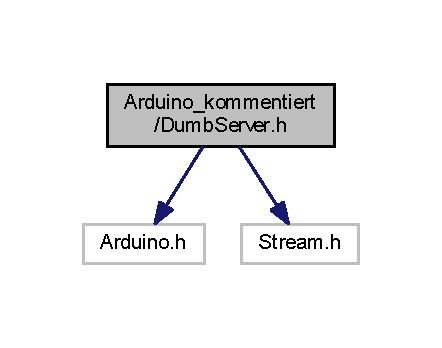
\includegraphics[width=212pt]{_dumb_server_8h__incl}
\end{center}
\end{figure}
Dieser Graph zeigt, welche Datei direkt oder indirekt diese Datei enthält\+:\nopagebreak
\begin{figure}[H]
\begin{center}
\leavevmode
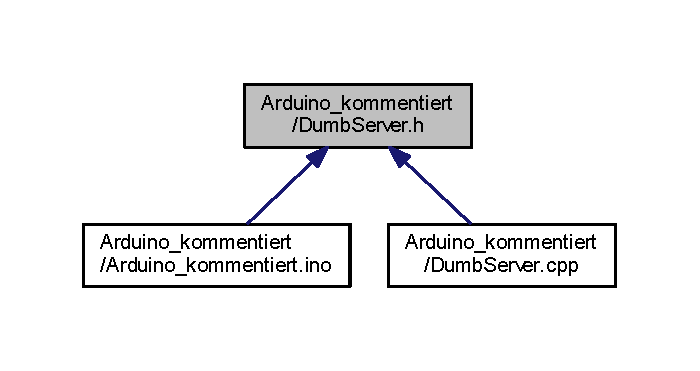
\includegraphics[width=336pt]{_dumb_server_8h__dep__incl}
\end{center}
\end{figure}
\subsection*{Datenstrukturen}
\begin{DoxyCompactItemize}
\item 
class \hyperlink{class_esp_server}{Esp\+Server}
\end{DoxyCompactItemize}

%--- End generated contents ---

% Index
\backmatter
\newpage
\phantomsection
\clearemptydoublepage
\addcontentsline{toc}{chapter}{Index}
\printindex

\end{document}
